\documentclass[final,3p,11pt,pdflatex]{elsarticle}
\usepackage[utf8x]{inputenc}      % input font encoding
\usepackage{amsmath,amssymb}
\usepackage[T1]{fontenc}          % output font encoding
\usepackage{booktabs,tabularx}
\usepackage{rotating}             % for sidewaystable
\usepackage{xspace}
\usepackage[usenames]{xcolor}
\usepackage{tikz,tikz-uml}
\usepackage{listings}
\bibstyle{elsarticle-num}
% source code highlighting
\lstset{breaklines=true,
  breakatwhitespace=true,
  stepnumber=1,
  basicstyle=\ttfamily\footnotesize,
  commentstyle=\ttfamily\color{gray},
  prebreak={\textbackslash},
  breakindent=10pt,
  breakautoindent=false,
  showspaces=false,
  showstringspaces=false,
  frame=single,
  abovecaptionskip=0em,
  aboveskip=1.5em,
  belowcaptionskip=0.5em,
  belowskip=1em,
}
\usepackage[pdftitle={FlexibleSUSY --- A spectrum generator generator for supersymmetric models},
pdfauthor={Peter Athron,Jae-hyeon Park,Dominik Stockinger,Alexander Voigt},
pdfkeywords={FlexibleSUSY,supersymmetry,spectrum,generator,MSSM,NMSSM,E6SSM},
bookmarks=true, linktocpage]{hyperref}

%macros
\newcommand{\sarah}{SARAH\@\xspace}
\newcommand{\fs}{FlexibleSUSY\@\xspace}
\newcommand{\mathematica}{Mathematica\xspace}
\newcommand{\ESSM}{E$_6$SSM\@\xspace}
\newcommand{\code}[1]{\lstinline|#1|}  % inline source code
\newcommand{\textoverline}[1]{$\overline{\mbox{#1}}$}
\newcommand{\DRbar}{\textoverline{DR}\xspace}
\newcommand{\MSbar}{\textoverline{MS}\xspace}
\newcommand{\unit}[1]{\,\text{#1}}      % units
\newcommand{\userinput}{\text{input}}
\newcommand{\pole}{\text{pole}}
\newcommand{\Lagr}{\mathcal{L}}
\newcommand{\unity}{\mathbf{1}}
\newcommand{\figref}[1]{\figurename~\ref{#1}}
\newcommand{\secref}[1]{Section~\ref{#1}}
\newcommand{\tabref}[1]{\tablename~\ref{#1}}
\newcommand{\ptitle}[1]{\emph{#1}}
\renewcommand{\ptitle}[1]{}
\newcommand{\JHtxt}[1]{\textcolor[rgb]{1,.3,0}{\texttt{#1}}}
\newcommand{\JHrem}[1]{\textcolor[rgb]{1,.3,0}{\textbf{{\textsl{\boldmath #1}}}}}
\makeatletter
\lstnewenvironment{numlstlisting}[1][]{%
  \lstset{%
    #1,
    numbers=left,
    firstnumber=auto,
    numberstyle=\tiny\sffamily}%
  \csname\@lst @SetFirstNumber\endcsname
}{%
  \csname \@lst @SaveFirstNumber\endcsname
}
\makeatother
\DeclareMathOperator{\diag}{diag}
\DeclareMathOperator{\sign}{sign}
\DeclareMathOperator{\re}{Re}
\DeclareMathOperator{\im}{Im}
\def\at{\alpha_t}
\def\ab{\alpha_b}
\def\as{\alpha_s}
\def\atau{\alpha_{\tau}}
\def\oat{O(\at)}
\def\oab{O(\ab)}
\def\oatau{O(\atau)}
\def\oatab{O(\at\ab)}
\def\oatas{O(\at\as)}
\def\oabas{O(\ab\as)}
\def\oatababq{O(\at\ab + \ab^2)}
\def\oatqatababq{O(\at^2 + \at\ab + \ab^2)}
\def\oatasatq{O(\at\as + \at^2)}
\def\oatasabas{O(\at\as +\ab\as)}
\def\oatasabasatq{O(\at\as + \at^2 +\ab\as)}
\def\oatq{O(\at^2)}
\def\oabq{O(\ab^2)}
\def\oatauq{O(\atau^2)}
\def\oabatau{O(\ab \atau)}
\def\oas{O(\as)}
\def\oatauqatab{O(\atau^2 +\ab \atau )}

\journal{Computer Physics Communications}
\begin{document}
\begin{frontmatter}

 \title{\Large\bf FlexibleSUSY --- A spectrum generator generator for supersymmetric models}

\author[adelaide]{Peter Athron}
\author[valencia]{Jae-hyeon Park}
\author[dresden]{Dominik St\"ockinger}
\author[dresden]{Alexander Voigt}
\address[adelaide]{ARC Centre of Excellence for Particle Physics at 
the Tera-scale, School of Chemistry and Physics, University of Adelaide, 
Adelaide SA 5005 Australia}
\address[valencia]{Departament de F\'{i}sica Te\`{o}rica and IFIC,
Universitat de Val\`{e}ncia-CSIC,
46100, Burjassot, Spain}
\address[dresden]{Institut f\"ur Kern- und Teilchenphysik,
TU Dresden, Zellescher Weg 19, 01069 Dresden, Germany}
   
  \begin{abstract}
   We introduce \fs, a \mathematica package which generates a fast,
   precise C++ spectrum generator for any SUSY model specified by the
   user.  The generated code is designed with both speed and
   modularity in mind, making it easy to adapt and extend with new
   features. The user specifies the model supplying the
   superpotential, gauge structure and particle content in a \sarah
   model file and provides the specific boundary conditions in a
   separate \fs model file. \fs makes use of the existing \sarah
   package to obtain self energies, tadpole corrections,
   renormalization group equations (RGEs) and tree level mass and
   electroweak symmetry breaking conditions for the specified model. These are
   translated into C++ code and combined  with numerical
   routines for solving the RGEs, EWSB conditions and simultaneously
   solving for the spectrum consistent with user specified boundary
   conditions.  The modular structure of the generated code allows for
   individual components to be replaced with an alternative if
   available. \fs has been carefully designed to grow as
   alternative solvers and calculators are added.
  \end{abstract}

\begin{keyword}
sparticle, 
supersymmetry, 
Higgs
\PACS 12.60.Jv
\PACS 14.80.Ly
\end{keyword}
\end{frontmatter}

\section{Program Summary}
\noindent{\em Program title:} \fs\\ {\em Program obtainable from:}
         {\tt http://flexiblesusy.hepforge.org/}\\ {\em Distribution
           format:}\/ tar.gz\\ {\em Programming language:} {\tt
           C++, \mathematica, FORTRAN}\\ {\em Computer:}\/ Personal computer\\ {\em Operating
           system:}\/ Tested on Linux 3.x, MacOS\\ {\em Word size:}\/ 64
         bits\\ {\em External routines:}\/ SARAH 4.0.4, Boost library,
         Eigen, LAPACK\\ {\em
           Typical running time:}\/ 0.1-0.3 seconds per parameter
         point.\\ {\em Nature of problem:}\/ Determining the mass
         spectrum and mixings for any supersymmetric model. The
         generated code must find simultaneous solutions to
         constraints which are specified at two or more different
         renormalization scales, which are connected by
         renormalization group equations forming a large set of
         coupled first-order differential equations. \\ {\em Solution method:}\/
         Nested iterative algorithm and numerical minimisation of the
         Higgs potential.  \\ {\em Restrictions:} The couplings must
         remain perturbative at all scales between the highest and
         lowest boundary condition.  \fs~ assumes that all couplings
         of the model are real (i.e.\ $CP-$conserving). Due to the
         modular nature of the generated code adaption and extension
         to overcome restrictions in scope is quite straightforward.





\newpage
\section{Introduction}
Supersymmetry (SUSY) provides the only non-trivial way to extend the
space-time symmetries of the Poincar\'e
group \cite{Coleman:1967ad,Haag:1974qh}, leading many to suspect that
SUSY may be realized in nature in some form. In particular
supersymmetric extensions of the standard model (SM) where SUSY is broken
at the TeV scale have been proposed to solve the hierarchy
problem \cite{Weinberg:1975gm, Weinberg:1979bn, Gildener:1976ai,
  Susskind:1978ms, 'tHooft:1980xb}, allow gauge coupling
unification \cite{Langacker:1990jh, Ellis:1990wk, Amaldi:1991cn,
  Langacker:1991an, Giunti:1991ta} and predict a dark matter candidate
which can fit the observed relic
density \cite{Goldberg:1983nd,Ellis:1983ew}.  Such models have also
been used for baryogenesis or leptogensis to solve the
matter-anti-matter asymmetry of the universe and have been considered
as the low energy effective models originating from string
theory.

Detailed phenomenological studies have been carried out for scenarios
within the minimal supersymmetric standard model (MSSM).  Such work
has been greatly aided by public spectrum generators for
MSSM \cite{Allanach:2001kg,Porod:2003um,Djouadi:2002ze,Baer:1993ae,Chowdhury:2011zr},
allowing fast and reliable exploration of the sparticle spectrum,
mixings and couplings, which can be obtained from particular choices
of breaking mechanism inspired boundary conditions and specified
parameters. Beyond the MSSM there are also two public spectrum
generators \cite{Ellwanger:2006rn,Allanach:2013kza} for the next to
minimal supersymmetric standard model (NMSSM) \cite{NMSSM}.

None of the fundamental motivations of supersymmetry require
minimality, and specific alternatives to (or extensions of) the MSSM
are, for example, motivated by the $\mu$-problem of the
MSSM \cite{Kim:1983dt}; explaining the family structure (see e.g.~\cite{King:2014nza}) or for successful baryogenesis or leptogenesis
(see e.g.~\cite{King:2008qb}). However constructing specialized tools
to study all relevant models would require an enormous amount of work.
So general tools which can automate this process and produce fast and
reliable programs can greatly enhance our ability to understand and
test non-minimal realizations of supersymmetry.

Recent experimental developments have also increased the relevancy of
such a tool. From the recent $7$ TeV and $8$ TeV runs at the Large
Hadron Collider (LHC) there have been two important developments.
First low energy signatures expected from such models, such as the
classic jets plus missing transverse energy signature, have not been
observed, substantially raising the lower limit on sparticle masses
(see e.g.~\cite{Aad:2013wta,Chatrchyan:2014lfa}). No other signature
of beyond the standard model (BSM) physics has been observed, leaving
the fundamental questions which motivated BSM physics
unanswered. Secondly ATLAS and CMS discovered \cite{ATLAS:2012ae,
  Chatrchyan:2012tx} a light Higgs of $125$ GeV, within the mass range
that could be accommodated in the MSSM but requiring stops which are
significantly heavier than both the direct collider limits and
indirect limits that appears in constrained models from the
significantly higher limits on first and second generation squarks.

These motivate both exploring non-minimal SUSY models which ameliorate
the naturalness problems by, for example, raising the tree level Higgs
mass and models developed with a fresh perspective based on other
considerations.  In both cases exploration of such models can be aided
if it is possible to quickly create a fast spectrum generator.
Currently there is only one option for this, a SPheno-like FORTRAN code
which can be generated from
\sarah \cite{Staub:2010ty,Staub:2009bi,Staub:2010jh,Staub:2012pb,Staub:2013tta}.

\fs provides a much needed alternative to this with a structure which
has been freshly designed to accommodate as general range of models as
possible and to be easily adaptable to changing goals and new
ideas. \fs is a \mathematica package which uses \sarah to create a
fast, modular C++ spectrum generator for a user specified SUSY model.
The generated code structure is designed to be as flexible as possible
to accommodate different types of extensions and due to its modular
nature it is easy to modify, add new features and combine with other
programs.  The generated code has been extensively tested against well
known spectrum generators. As well as providing a solution for new
SUSY models, the generated MSSM and NMSSM codes offer a modern and fast
alternative to the existing public spectrum generators.

In \secref{sec:Program} we describe the program in more detail and
explain our design goals.  In \secref{sec:download} information on how
to download and compile the code may be found along with details on
how to get started quickly.  In \secref{sec:modfile} we describe how
the user can create a new FlexibleSUSY model file. A detailed
description of the structure and features of the generated code is
then given in \secref{sec:SpecGenStruct}.  In \secref{sec:Flexible} we
describe the various ways the code can be modified both at the meta
code level by writing model files and at the C++ code level by
modifying the code or adding new modules. Finally in
\secref{sec:comparison} we describe detailed comparisons between our
generated code and existing public spectrum generators as well as
against the SPheno-like FORTRAN code which can be created using SARAH.


\section{Overview of the program and design goals}
\label{sec:Program}

To study the properties of SUSY models programs are needed which
numerically calculate the pole masses and couplings of the SUSY
particles given a set of theory input parameters.  The output of these
so-called spectrum generators can be transferred to programs which
calculate further observables such as branching rations or the dark
matter relic density.

In order to create a spectrum generator the SUSY model must be defined
by specifying the gauge group, the field content and mixings as well
as the superpotential and the soft-breaking terms.  From this
information the renormalization group equations, mass matrices,
self-energies, tadpole diagrams and electroweak symmetry breaking
(EWSB) conditions have to be derived.  These expressions must then be
combined in a computer program to allow for a numeric calculation of
the mass spectrum.  In addition most SUSY models require boundary
conditions for the model parameters at a low and a high scale.  For
example in the CMSSM mSUGRA boundary conditions for the soft-breaking
parameters are imposed at the gauge coupling unification scale.
Furthermore, at the $Z$ mass scale the CMSSM is matched to the Standard
Model, which implies conditions for the gauge and Yukawa couplings.
The so defined boundary value problem must be solved numerically until
a set of model parameters has been found consistent with all
user-supplied boundary conditions.

\fs is a \mathematica package designed to create a fast and easily
adaptable spectrum generator in C++ for any SUSY model.
The user specifies the model by giving the
superfield content, superpotential, gauge symmetries and mass mixings
in form of \sarah model files.  The boundary conditions on the model
parameters must be specified in a separate \code{FlexibleSUSY.m} file.
Based on this information \fs uses \sarah to obtain tree-level
expressions for the mass matrices and electroweak symmetry breaking
conditions, one-loop self energies, one-loop tadpoles corrections and
two-loop renormalisation group equations (RGEs) for the model.
Additional corrections which have been calculated elsewhere, such as
two-loop corrections to the Higgs masses\footnote{By default
  FlexibleSUSY has two-loop corrections to the Higgs masses for the
  MSSM
  \cite{Degrassi:2001yf,Brignole:2001jy,Dedes:2002dy,Brignole:2002bz,Dedes:2003km}
  and NMSSM \cite{Degrassi:2009yq} in FORTRAN files supplied by Pietro
  Slavich. These are the same corrections which are implemented in
  many of the public spectrum generators.} may be added by the user.
%
These algebraic expressions are converted into C++ code and are put
into classes with well-defined interfaces to allow for easy exchange,
extension and reuse of the modules.  All of these classes are finally
combined to a complete spectrum generator, which solves the
user-defined boundary value problem.  For this task \fs uses some
parts of Softsusy \cite{Allanach:2001kg}, the very fast Eigen library
\cite{eigen}, augmented by LAPACK, as well as the GNU scientific
library and the BOOST library to create numerical routines which solve
the RGEs and boundary conditions simultaneously.  If a solution has
been found the pole mass spectrum is eventually calculated using full
one-loop self-energies (and leading two-loop Higgs self-energy
contributions for the MSSM and NMSSM).

\subsection*{Design goals}

Since the calculation of the pole mass spectrum in a SUSY model is a
non-trivial task, \fs is designed with the following points in mind:

\paragraph{Modularity}

The large variety of supersymmetric models and potential
investigations makes it likely that the user wants to modify the
generated spectrum generator source code or reuse components in
further programs.  \fs offers two levels to influence the code: (i) On
the \mathematica model file level the model itself or GUT/weak scale
boundary conditions as well as input and output parameters can be
controlled (see \secref{sec:quick-start-alternative-models} and
\secref{sec:adapting-model-files} for examples).  (ii) In particular
\fs uses C++ object orientation features to modularize the source code
in order to make it easy for the user to modify, reuse, replace or
extend the individual components (see \secref{sec:adapting-cpp-code}
for examples).  An important application of this concept are the
boundary conditions, for which the C++ level offers a wider range of
possibilities.  The boundary conditions solver provides a plugin
mechanism via a common \code{Constraint} interface, which allows a
user to exchange or add boundary conditions at any scale.  An
elaborate example of a tower of effective field theories and multiple
matching scales is presented in \secref{sec:tower construction}.
Alternatively, the modular structure makes it straightforward to take
\fs generated code for e.g.\ RGEs or self-energies and reuse it in an
existing code for some other purpose.  Conversely, it is also easy to
include code from elsewhere into the spectrum generator.  For an
example see \secref{sec:integrating-custom-built}.

\paragraph{Speed}

Exploring the parameter space of supersymmetric models with a high
number of free parameters is quite time consuming.  Therefore \fs aims
to produce spectrum generators with a short run-time.  The two most
time consuming parts of a SUSY spectrum generator are usually the
calculation of the two-loop $\beta$-functions and the pole masses of
mixed particles:
%
\begin{itemize}
\item \emph{Calculation of the $\beta$-functions:} The RG solving
  algorithms usually need $O(10)$ iterations between the high and the
  low scale to find a set of parameters consistent will all boundary
  conditions with a $0.01\%$ precision goal.  During each iteration
  the Runge-Kutta algorithm needs to calculate all $\beta$-functions
  $O(50)$ times.  Most two-loop $\beta$-functions involve $O(50)$
  matrix multiplications and additions.  All together one arrives at
  $O(10^4)$ matrix operations.  To optimize these, \fs uses the fast
  linear algebra package \href{Eigen}{http://eigen.tuxfamily.org}.
  Eigen uses C++ expression templates to remove temporary objects and
  enable lazy evaluation of the expressions.  It supports explicit
  vectorization, and provides fixed-size matrices to avoid dynamic
  memory allocation.  All of these features in combination result in
  very fast code for the calculation of the $\beta$-functions in \fs.
%
\item \emph{Calculation of the pole masses:} The second most time
  consuming part is the precise calculation of the pole masses for
  mixed particles.  For each particle $\psi_k$ in a multiplet the full
  self-energy matrix $\Sigma^\psi_{ij}(p=m^\text{tree}_{\psi_k})$ has
  to be evaluated.  Each self-energy matrix entry again involves the
  calculation of $O(50)$ Feynman diagrams, each involving the
  calculation of vertices and a loop-function.  All in all, one
  arrives at $O(500)$ Feynman diagrams and $O(10^4)$ loop function
  evaluations.  To speed up the calculation of the pole masses \fs
  makes use of multi-threading, where each pole mass is calculated in
  a separate thread.  This allows the operating system to distribute
  these calculations among different CPU cores.  With this technique
  one can gain a speed-up of $20$--$30\%$.
\end{itemize}

\paragraph{Alternative boundary value problem solvers}

Furthermore, the standard algorithm which solves the user-defined
boundary value problem via a fixed-point iteration is not guaranteed
to converge in all regions of the model parameter space.  Therefore,
\fs has been intentionally designed to allow for alternative solvers
to search for solutions in such critical parameter regions.  A
subsequent release with an alternative solver is already planned.

\paragraph{Towers of effective theories}

In \fs the standard fixed-point iteration solver has been generalized
to handle towers of models (effective theories), which are matched at
intermediate scales.  An example of such a tower construction will be
given in \secref{sec:tower construction}, where right-handed neutrinos
are integrated out at the see-saw scale, between the SUSY and the GUT
scale.

\section{Quick start}
\label{sec:download}

\subsection{Requirements}

\fs can be downloaded from \url{http://flexiblesusy.hepforge.org}.  To
create a custom spectrum generator the following requirements are
necessary:
%
\begin{itemize}
\item \mathematica, version 7 or higher
\item SARAH, version 4.0.4 or higher \url{http://sarah.hepforge.org}
\item C++11 compatible compiler (g++ 4.4.7 or higher, clang++ 3.1 or
  higher, icpc 12.1 or higher)
\item FORTRAN compiler (gfortran, ifort etc.)
\item Eigen library, version 3.1 or higher
  \url{http://eigen.tuxfamily.org}
\item Boost library, version 1.36.0 or higher
  \url{http://www.boost.org}
\item GNU scientific library \url{http://www.gnu.org/software/gsl/}
\item an implementation of LAPACK \url{http://www.netlib.org/lapack/}
  such as ATLAS \url{http://math-atlas.sourceforge.net/} or
  Intel Math Kernel Library \url{http://software.intel.com/intel-mkl}
\end{itemize}
%
Optional:
%
\begin{itemize}
\item Looptools, version 2.8 or higher
  \url{http://www.feynarts.de/looptools/}
\end{itemize}

\subsection{Download and generating a first spectrum generator}
\label{sec:quick-start-cmssm}

\fs can be downloaded as a gzipped tar file from
\url{http://flexiblesusy.hepforge.org/}.  To download and install
version 1.0.0 run:
%
\begin{lstlisting}[language=bash]
$ wget https://www.hepforge.org/archive/flexiblesusy/FlexibleSUSY-1.0.0.tar.gz
$ tar -xf FlexibleSUSY-1.0.0.tar.gz
$ cd FlexibleSUSY-1.0.0/
\end{lstlisting}%% $
%
A CMSSM spectrum generator can be created with the following three
commands:
%
\begin{lstlisting}[language=bash]
$ ./createmodel --name=MSSM
$ ./configure --with-models=MSSM
$ make
\end{lstlisting}%% $
%
The first command creates the model directory \code{models/MSSM/}
together with a CMSSM model file.  The \code{configure} script checks
the system requirements and creates the \code{Makefile}.  See
\code{./configure --help} for more options.  Executing \code{make}
will start \mathematica to generate the spectrum generator and compile
it.  The resulting executable can be run like this:
%
\begin{lstlisting}[language=bash]
$ models/MSSM/run_MSSM.x \
    --slha-input-file=model_files/MSSM/LesHouches.in.MSSM
\end{lstlisting}%% $
%
When executed, the spectrum generator tries to find a set of \DRbar\
model parameters consistent with all CMSSM boundary conditions for the
parameter point given in the SLHA input file
\code{model_files/MSSM/LesHouches.in.MSSM}.  Afterwards, the pole mass
spectrum and mixing matrices are calculated and written to the command
line in SLHA format \cite{Skands:2003cj,Allanach:2008qq}.  For the
parameter point given in the above example the calculated pole mass
spectrum reads
%
\begin{lstlisting}
Block MASS
   1000021     1.15236966E+03   # Glu
   1000024     3.85774334E+02   # Cha_1
   1000037     6.50460073E+02   # Cha_2
        25     1.14766149E+02   # hh_1
        35     7.06792640E+02   # hh_2
        37     7.11388516E+02   # Hpm_2
        36     7.06523105E+02   # Ah_2
   1000012     3.51856376E+02   # Sv_1
   1000014     3.53042556E+02   # Sv_2
   1000016     3.53046504E+02   # Sv_3
   1000022     2.03889780E+02   # Chi_1
   1000023     3.85760714E+02   # Chi_2
   1000025     6.36544884E+02   # Chi_3
   1000035     6.50133768E+02   # Chi_4
   1000001     9.66656018E+02   # Sd_1
   1000003     1.00983181E+03   # Sd_2
   1000005     1.01651873E+03   # Sd_3
   2000001     1.01653005E+03   # Sd_4
   2000003     1.06089534E+03   # Sd_5
   2000005     1.06090238E+03   # Sd_6
   1000011     2.22570305E+02   # Se_1
   1000013     2.29864536E+02   # Se_2
   1000015     2.29888846E+02   # Se_3
   2000011     3.61946671E+02   # Se_4
   2000013     3.61950866E+02   # Se_5
   2000015     3.63136031E+02   # Se_6
   1000002     8.09787818E+02   # Su_1
   1000004     1.01454197E+03   # Su_2
   1000006     1.01981109E+03   # Su_3
   2000002     1.02015269E+03   # Su_4
   2000004     1.05807759E+03   # Su_5
   2000006     1.05808168E+03   # Su_6
\end{lstlisting}

\subsection{Spectrum generators for alternative models}
\label{sec:quick-start-alternative-models}

\fs already comes with plenty of predefined models: the CMSSM (simply
called \code{MSSM}), the $Z_3$-symmetric NMSSM (called \code{NMSSM})
\cite{Ellwanger:2009dp}, $Z_3$-violating NMSSM (\code{SMSSM})
\cite{Ellwanger:2009dp}, the USSM (\code{UMSSM})
\cite{Fayet:1977yc,Cvetic:1997ky,Erler:2002pr}, the NUHM-\ESSM
(\code{E6SSM}) \cite{King:2005jy,Athron:2007en}, the right-handed
neutrino extended MSSM (\code{MSSMRHN}), the NUHM-MSSM
(\code{NUHMSSM}) and the $R$-symmetric MSSM (\code{MRSSM})
\cite{Kribs:2007ac}.  See the content of \code{model_files/} for all
predefined model files.  For all these models spectrum generators can
be generated easily like for the CMSSM in
\secref{sec:quick-start-cmssm}.  The spectrum generator for the
$Z_3$-symmetric NMSSM for example can be generated like this:
%
\begin{lstlisting}[language=bash]
$ ./createmodel --name=NMSSM
$ ./configure --with-models=NMSSM
$ make
\end{lstlisting}%% $
%
One of the design goals is modularity and the possibility to easily
construct custom spectrum generators.  The details of the
customization can be found in Sections
\ref{sec:modfile}--\ref{sec:Flexible}.  As a simple example consider
the NMSSM.  The NMSSM variant above unifies all soft-breaking
trilinear scalar couplings at the GUT scale.  In order to relax this
constraint and use a separate value for $A_\lambda$ at the GUT scale
one can edit the model file \code{models/NMSSM/FlexibleSUSY.m} and
change the lines
%
\begin{lstlisting}[language=Mathematica]
EXTPAR = { {61, LambdaInput} };

HighScaleInput = {
   ...
   {T[\[Lambda]], Azero LambdaInput},
   ...
};
\end{lstlisting}
%
into
%
\begin{lstlisting}[language=Mathematica]
EXTPAR = { {61, LambdaInput},
           {63, ALambdaInput} };

HighScaleInput = {
   ...
   {T[\[Lambda]], ALambdaInput LambdaInput},
   ...
};
\end{lstlisting}
%
The value of $A_\lambda$ at the GUT scale can then be set in the SLHA
input file in the \code{EXTPAR} block entry $63$ via
%
\begin{lstlisting}
Block EXTPAR
   61   0.1                  # LambdaInput
   63   -100                 # ALambdaInput
\end{lstlisting}

\section{Setting up a FlexibleSUSY model}
\label{sec:modfile}

A general (non-constrained) softly broken SUSY model is defined by the
gauge group, the field content and mixings as well as the
superpotential and the soft-breaking Lagrangian.  In order to create a
spectrum generator for such a SUSY model with \fs, the aforementioned
model properties have to be defined in a SARAH model file.  The SARAH
model file can be put into the \code{sarah/<model>/} directory.  See
the SARAH manual \cite{Staub:2008uz,Staub:2013tta} for a detailed
explanation of how to write such a model file.  Note that SARAH
already comes with a lot of predefined models, which can be used with
\fs immediately.

The model boundary conditions are defined in the \fs model file
\code{FlexibleSUSY.m}, which has to be located in the model directory
\code{models/<model>/}.  Note that many example model files can
already be found in \code{model_files/}.  In the following it is
explained how the boundary conditions can be defined on the basis of
the CMSSM.  The application to other models is straightforward.  The
CMSSM model file reads:
%
\begin{lstlisting}[language=Mathematica]
FSModelName = "MSSM";

MINPAR = {
   {1, m0},
   {2, m12},
   {3, TanBeta},
   {4, Sign[\[Mu]]},
   {5, Azero}
};

EWSBOutputParameters = { B[\[Mu]], \[Mu] };

HighScale = g1 == g2;

HighScaleFirstGuess = 2.0 10^16;

HighScaleMinimum = 1.0 10^10; (* optional *)

HighScaleMaximum = 1.0 10^18; (* optional *)

HighScaleInput = {
   {T[Ye], Azero*Ye},
   {T[Yd], Azero*Yd},
   {T[Yu], Azero*Yu},
   {mHd2, m0^2},
   {mHu2, m0^2},
   {mq2, UNITMATRIX[3] m0^2},
   {ml2, UNITMATRIX[3] m0^2},
   {md2, UNITMATRIX[3] m0^2},
   {mu2, UNITMATRIX[3] m0^2},
   {me2, UNITMATRIX[3] m0^2},
   {MassB, m12},
   {MassWB, m12},
   {MassG, m12}
};

SUSYScale = Sqrt[M[Su[1]]*M[Su[6]]];

SUSYScaleFirstGuess = Sqrt[m0^2 + 4 m12^2];

SUSYScaleInput = {};

LowScale = SM[MZ];

LowScaleFirstGuess = SM[MZ];

LowScaleInput = {
   {Yu, Automatic},
   {Yd, Automatic},
   {Ye, Automatic},
   {vd, 2 MZDRbar / Sqrt[GUTNormalization[g1]^2 g1^2 + g2^2]
           Cos[ArcTan[TanBeta]]},
   {vu, 2 MZDRbar / Sqrt[GUTNormalization[g1]^2 g1^2 + g2^2]
           Sin[ArcTan[TanBeta]]}
};

InitialGuessAtLowScale = {
   {vd, SM[vev] Cos[ArcTan[TanBeta]]},
   {vu, SM[vev] Sin[ArcTan[TanBeta]]},
   {Yu, Automatic},
   {Yd, Automatic},
   {Ye, Automatic}
};

InitialGuessAtHighScale = {
   {\[Mu]   , 1.0},
   {B[\[Mu]], 0.0}
};

UseHiggs2LoopMSSM = True;
EffectiveMu = \[Mu];

OnlyLowEnergyFlexibleSUSY = False; (* default *)

PotentialLSPParticles = { Chi, Cha, Glu, Sv, Su, Sd, Se };

DefaultPoleMassPrecision = MediumPrecision;
HighPoleMassPrecision    = {hh, Ah, Hpm};
MediumPoleMassPrecision  = {};
LowPoleMassPrecision     = {};
\end{lstlisting}
%
The variable \code{FSModelName} contains the name of the \fs model.

All non-Standard Model input variables must be specified in the lists
\code{MINPAR} and \code{EXTPAR}.  These two variables refer to the
MINPAR and EXTPAR blocks in a SLHA input file \cite{Skands:2003cj}.
The list elements are two-component lists where the first entry is the
SLHA index in the MINPAR or EXTPAR block, respectively, and the second
entry is the name of the input parameter.  In the above example the
input parameters are the universal soft-breaking parameters $m_0$,
$M_{1/2}$, $A_0$ as well as $\tan\beta$ and $\sign\mu$.

Using the the variable \code{EWSBOutputParameters} the user can
specify the model parameters that are output of the electroweak
symmetry breaking consistency conditions.  When imposing the EWSB, \fs
will adjust these parameters until the EWSB conditions are fulfilled.
In the CMSSM example above these are the superpotential parameter
$\mu$ and its corresponding soft-breaking parameter $B\mu$.  In the
NMSSM the parameters $\kappa$, $|v_s|$ and $m_s^2$ are usually chosen
for this purpose.

Furthermore, the user has to specify three model constraints:
low-scale, SUSY-scale and high-scale.  In \fs they are named as
\code{LowScale}, \code{SUSYScale} and \code{HighScale}.  For each
constraint there is (i) a scale definition (named after the
constraint), (ii) an initial guess for the scale (concatenation of the
constraint name and \code{FirstGuess}) and (iii) a list of parameter
settings to be applied at the scale (concatenation of the constraint
name and \code{Input}).  Optionally a minimum and a maximum value for
the scale can be given (concatenation of the constraint name and
\code{Minimum} or \code{Maximum}, respectively).  The latter avoids
underflows or overflows of the scale value during the iteration.  This
is especially useful in models where the iteration is very unstable
and the value of the scale is very sensitive to the model parameters.
The meaning of the three constraints is the following:
%
\begin{itemize}
\item \emph{High-scale constraint:} The high-scale constraint is
  usually the GUT-scale constraint, imposed at the scale where the
  gauge couplings $g_1$ and $g_2$ unify.  The high-scale can be
  defined by an equation of the form \code{g1 == g2} or by a fixed
  numerical value.  Note that \fs GUT-normalizes all gauge couplings.
  Thus, the high-scale definition takes the simple form \code{g1 ==
    g2}.  As a consequence in the calculation of the VEVs $v_u$ and
  $v_d$ from $M_Z$ and $\tan\beta$ at the low-scale the
  GUT-normalization has to be taken into account, see the example
  above.
%
\item \emph{SUSY-scale constraint:} The SUSY-scale is the typical mass
  scale of the SUSY particle spectrum.  At this scale \fs imposes the
  EWSB conditions and calculates the pole mass spectrum.  The
  SUSY-scale, $M_S$, is usually defined as $M_S =
  \sqrt{m_{\tilde{t}_1}m_{\tilde{t}_2}}$.  However, in the example
  above, where sfermion flavour violation is enabled, it has the value
  $M_S = \sqrt{m_{\tilde{u}_1}m_{\tilde{u}_6}}$, where
  $m_{\tilde{u}_1}$ and $m_{\tilde{u}_6}$ are the \DRbar\ masses of
  the lightest and heaviest up-type squark, respectively.
%
\item \emph{Low-scale constraint:} The low-scale constraint is the
  constraint where the SUSY model is matched to the Standard Model.
  This is done by automatically calculating the gauge couplings $g_i$
  ($i=1,2,3$) of the SUSY model from the known Standard Model
  quantities $\alpha_{\text{e.m.}}(M_Z)$, $\alpha_{s}(M_Z)$, $M_Z$,
  $M_W$.  The details of this calculation are explained in
  \secref{sec:calculation-of-gauge-couplings}.  Currently this scale
  is fixed to be the $Z$ pole mass scale $M_Z$.  Optionally the Yukawa
  couplings $y_f$ ($f=u,d,e$) can be calculated automatically from the
  known Standard Model fermion masses $m_f$ by setting their values to
  \code{Automatic}.  This automatic calculation is explained in
  \secref{sec:calculation-of-yukawa-couplings}.
\end{itemize}
%
The variables \code{LowScaleInput}, \code{SUSYScaleInput}
\code{HighScaleInput}, which list the parameter settings for imposing
the constraints can contain as elements any of the following:
%
\begin{itemize}
\item Two-component lists of the form \code{\{parameter, value\}},
  which indicates that the \code{parameter} is set to \code{value} at
  the defined scale.  If the \code{value} should be read from the SLHA
  input file, it must be written as \code{LHInput[value]}.  Example:
  %
  \begin{lstlisting}
SUSYScaleInput = {
   {mHd2, m0^2},
   {mHu2, LHInput[mHu2]}
};
  \end{lstlisting}
  %
  In this example the parameter \code{mHd2} is set to the value of
  \code{m0^2}, and \code{mHu2} is set to the value given in the SLHA
  input file in block \code{MSOFTIN}, entry 22 at the SUSY scale.  The
  SLHA block names and keys for the MSSM and NMSSM are defined in
  SARAH's \code{parameters.m} file, see the SARAH manual or
  \cite{Staub:2010jh}.  For the Standard Model Yukawa couplings
  \code{Yu}, \code{Yd}, \code{Ye} the value \code{Automatic} is
  allowed, which triggers their automatic determination from the known
  Standard Model quark and lepton masses, see
  \secref{sec:calculation-of-yukawa-couplings}.

\item The function \code{FSMinimize[parameters, function]} can be
  given, where \code{parameters} is a list of model parameters and
  \code{function} is a function of these parameters.
  \code{FSMinimize[parameters, function]} will numerical vary the
  \code{parameters} until the \code{function} is minimized.  Example:
  %
  \begin{lstlisting}
FSMinimize[{vd,vu},
           (SM[MZ] - Pole[M[VZ]])^2 / STANDARDDEVIATION[MZ]^2 +
           (SM[MH] - Pole[M[hh[1]]])^2 / STANDARDDEVIATION[MH]^2]
  \end{lstlisting}
  %
  Here, the parameters \code{vu} and \code{vd} are varied until the
  function
  %
  \begin{align}
    \chi^2(v_d,v_u) =
    \frac{(\texttt{SM[MZ]}-m_Z^\pole)^2}{\sigma_{m_Z}^2} +
    \frac{(\texttt{SM[MH]}-m_{h_1}^\pole)^2}{\sigma_{m_h}^2}
  \end{align}
  %
  is minimal.  The constants \code{SM[MZ]}, \code{SM[MH]},
  $\sigma_{m_Z}$ and $\sigma_{m_h}$ are defined in
  \code{src/ew_input.hpp} to be
  %
  \begin{align}
    \texttt{SM[MZ]} &= 91.1876, &
    \texttt{SM[MH]} &= 125.9, \\
    \sigma_{m_Z} &= 0.0021, &
    \sigma_{m_h} &= 0.4 .
  \end{align}

\item The function \code{FSFindRoot[parameters, functions]} can be
  given, where \code{parameters} is a list of model parameters and
  \code{functions} is a list of functions of these parameters.
  \code{FSFindRoot[parameters, functions]} will numerical vary the
  \code{parameters} until the \code{functions} are zero.  Example:
  %
  \begin{lstlisting}
FSFindRoot[{vd,vu},
           {SM[MZ] - Pole[M[VZ]], SM[MH] - Pole[M[hh[1]]]}]
  \end{lstlisting}
  %
  Here, the parameters \code{vu} and \code{vd} are varied until the
  vector-like function
  %
  \begin{align}
    f(v_d,v_u) =
    \begin{pmatrix}
      \texttt{SM[MZ]} - m_Z^\pole \\
      \texttt{SM[MH]} - m_{h_1}^\pole
    \end{pmatrix}
  \end{align}
  %
  is zero.
\end{itemize}
%
Finally, the user can set an initial guess for the model parameters at
the low- and high-scale using the variables
\code{InitialGuessAtLowScale} and \code{InitialGuessAtHighScale},
respectively.  The gauge couplings will be guessed automatically at
the low-scale from the known Standard Model parameters.

\fs allows to add leading two-loop contributions to the CP-even Higgs
tadpoles and self-energies.  For MSSM-like models (with two CP-even
Higgs bosons, one CP-odd Higgs boson, one neutral Goldstone boson)
these corrections can be enabled by setting \code{UseHiggs2LoopMSSM =
  True} in the model file and by defining the effective $\mu$-term
\code{EffectiveMu = \\[Mu]}.  This will add the zero-momentum
corrections of the order $O(y_t^4 + y_b^2 y_t^2 + y_b^4)$, $O(y_t^2
g_3^2)$, $O(y_b^2 g_3^2)$, $O(y_\tau^4)$, $O(y_\tau^2 y_b^2)$ from
\cite{Degrassi:2001yf,Brignole:2001jy,Dedes:2002dy,Brignole:2002bz,Dedes:2003km}.
For NMSSM-like models (with three CP-even Higgs bosons, two CP-odd
Higgs bosons, one neutral Goldstone boson) the two-loop contributions
are enabled by setting \code{UseHiggs2LoopNMSSM = True} and by
defining the effective $\mu$-term like \code{EffectiveMu = \\[Lambda]
  vS / Sqrt[2]}, for example.  This will add the the zero-momentum
corrections of the order $O(y_t^2 g_3^2)$, $O(y_b^2 g_3^2)$ from
\cite{Degrassi:2009yq}, plus MSSM-like contributions of the order
$O(y_\tau^4)$, $O(y_t^4 + y_t^2 y_b^2 + y_b^4)$
\cite{Brignole:2001jy,Dedes:2003km}.

One can create a pure low-energy model by setting
\code{OnlyLowEnergyFlexibleSUSY = True}.  In this case the high-scale
constraint is ignored and only the low-scale and SUSY-scale
constraints are used.  All model parameters which are not specified in
\code{MINPAR} or \code{EXTPAR} will then be read from the
corresponding input blocks in the SLHA input file and will be set at
the SUSY-scale.  An example of such a pure low-energy model is the
MRSSM, where the three gauge couplings do not unify at a common scale.

\fs can create the helper function \code{get_lsp()}, which finds the
lightest supersymmetric particle (LSP).  To have this function be
created the model file variable \code{PotentialLSPParticles} must be
set to a list of SUSY particles which are potential LSPs.  In the
model file example above, the particles \code{Chi}, \code{Cha},
\code{Glu}, \code{Sv}, \code{Su}, \code{Sd}, \code{Se} (neutralino,
chargino, gluino, sneutrino, up-type squark, down-type squark,
selectron) are considered to be LSPs.

\section{Structure of the spectrum generator}
\label{sec:SpecGenStruct}

In this section we explain the internals of \fs's automatically
generated spectrum generator.

As mentioned in \secref{sec:Program}, \fs uses SARAH-generated
expressions for the $\beta$-functions, mass matrices, self-energies
and EWSB conditions plus the user-defined parameter boundary
conditions to create a spectrum generator in C++.  This program takes
the Standard Model and user-defined input parameters and numerically
solves the boundary value problem, which is defined by the RG
equations and the boundary conditions.  If a solution is found the
pole mass spectrum is calculated.

In the following it is explained how this procedure is realized in
\fs.  As mentioned in \secref{sec:Program} one of \fs's design goals
is to create modular C++ code to allow for an easy exchange, extension
and reuse of the generated modules.  For this reason
\secref{sec:ModelParametersAndRGEs} first of all briefly describes the
so-called C++ ``model class'' hierarchy, which contains the general
model information, such as parameters, $\beta$-functions, \DRbar\ mass
spectrum, EWSB, self-energies, and the pole mass spectrum.
%
\secref{sec:boundary-conditions} describes how boundary conditions on
the model parameters are implemented in general at the C++ level.
Subsections \ref{sec:calculation-of-gauge-couplings}--\ref{sec:ewsb}
then show the two concrete boundary conditions, which are always
imposed: The matching of the model parameters to the Standard Model
and the electroweak symmetry breaking.
%
In \secref{sec:TreeLevelSpectrum} we describe the conventions used to
calculate the \DRbar\ mass spectrum given a set of \DRbar\ model
parameters.
%
Afterwards, in \secref{sec:TwoScaleFixedPointIteration} the algorithm,
which solves the user-defined boundary value problem is described on
the basis of the CMSSM example given in \secref{sec:modfile}.
%
Finally, \secref{sec:PoleMasses} explains how the pole mass spectrum
is obtained from the \DRbar\ model parameters after a solution to the
boundary value problem has been found.

\subsection{Model parameters and RGEs}
\label{sec:ModelParametersAndRGEs}

The parameters of the SUSY model together with their RGEs, mass
matrices, self-energies and EWSB equations are stored at the C++ level
in the model class hierarchy, which is shown in the UML diagram in
\figref{fig:parameter-classes}.
%
\begin{figure}
  \centering
  \tikzumlset{fill class=white}
  \begin{tikzpicture}
    \umlclass[x=0, y=8, type=abstract]{Beta\_function}{
    }{
      + \umlvirt{get()}\\
      + \umlvirt{set()}\\
      + \umlvirt{beta()}\\
      + run\_to()
    }
    \umlclass[x=0, y=4]{<model>\_susy\_parameters}{
      -- susy parameters
    }{
      + get()\\
      + set()\\
      + beta()\\
      + run\_to()
    }
    \umlclass[x=0, y=0]{<model>\_soft\_parameters}{
      -- soft-breaking parameters
    }{
      + get()\\
      + set()\\
      + beta()\\
      + run\_to()
    }
    \umlclass[x=0, y=-3.5]{<model>}{}{
      + calculate\_spectrum()\\
      + solve\_ewsb()
    }
    \umlinherit{<model>\_susy\_parameters}{Beta\_function}
    \umlinherit{<model>\_soft\_parameters}{<model>\_susy\_parameters}
    \umlinherit{<model>}{<model>\_soft\_parameters}
  \end{tikzpicture}
  \caption{Model class hierarchy.}
  \label{fig:parameter-classes}
\end{figure}

The top of the hierarchy is formed by the \code{Beta_function}
interface class, which defines the basic RGE running interface.  It
provides the interface function \code{run_to()}, which integrates the
RGEs up to a given scale using an adaptive Runge-Kutta algorithm.
This algorithm uses the pure virtual functions \code{get()},
\code{set()} and \code{beta()}, which need to be implemented by a
derived class.  The \code{get()} and \code{set()} functions return and
set the model parameters in form of a vector, respectively.  The
\code{beta()} method returns the $\beta$-function for each parameter
in form of a vector as well.

All SUSY model parameters and their $\beta$-functions are contained in
the first and second derived classes.  The structure of the
$\beta$-functions of a general SUSY model
\cite{Jones:1974pg,Jones:1983vk,West:1984dg,Martin:1993yx,Yamada:1993ga,MV94,Fonseca:2011vn,Sperling:2013eva,Sperling:2013xqa}
allows to split these parameters into two classes:
%
\begin{enumerate}
\item \emph{SUSY parameters:} gauge couplings, superpotential
  parameters and VEVs and
\item \emph{soft-breaking parameters} \cite{Girardello:1981wz}: soft
  linear scalar terms, soft bilinear scalar interactions, soft
  trilinear scalar interactions, soft gaugino mass terms and soft
  scalar squared masses.
\end{enumerate}
%
The $\beta$-functions of the SUSY parameters in general depend only on
the SUSY parameters and are independent of the soft-breaking
parameters.  However, the $\beta$-functions of the soft-breaking
parameters depend on all model parameters in general.
%
This property is reflected in the C++ code: The class
\code{<model>_susy_parameters} directly inherits from
\code{Beta_functions} and implements the $\beta$-functions of the SUSY
parameters.  The class of soft-breaking parameters
\code{<model>_soft_parameters} in turn inherits from
\code{<model>_susy_parameters} and implements the $\beta$-functions of
the soft-breaking parameters in terms of all model parameters.  The so
constructed class hierarchy allows to (i) use the RGE running of all
model parameters via the common \code{Beta_function} interface and to
(ii) run the SUSY parameters independently of the soft-breaking
parameters.

\fs creates these two classes from the model parameters defined in the
SARAH model file.  The corresponding one- and two-loop
$\beta$-functions are calculated algebraically using SARAH's
\code{CalcRGEs[]} routine, converted to C++ form and written into the
corresponding \code{beta()} functions.  These two classes then allow
to use renormalization group running of all SUSY model parameters.

At the bottom of the hierarchy stands the actual model class, which
defines \code{calculate_spectrum()} and \code{solve_ewsb()} functions.
The former uses the mass matrices and self-energies obtained from
SARAH to calculate the pole mass spectrum.  It will be explained in
detail in \secref{sec:PoleMasses}.  The \code{solve_ewsb()} function
numerically solves the electroweak symmetry breaking equations and
will be explained in the next section.

\subsection{Boundary conditions}
\label{sec:boundary-conditions}

% The parameters of a SUSY model have to meet certain boundary
% conditions.  For example, the running gauge and Yukawa couplings
% should match the ones of the Standard Model at the scale $M_Z$.
% Usually also high-scale boundary conditions on the soft-breaking
% parameters are applied, as for example in mSUGRA scenarios.

As described in \secref{sec:modfile}, the user defines three boundary
conditions in the \fs model file at the \mathematica level.  These
boundary conditions are converted to C++ form and are put into
classes, which implement the common \code{Constraint<Two\_scale>}
interface.  This interface has the form:
%
\begin{lstlisting}[language=C++]
template<>
class Constraint<Two_scale> {
public:
   virtual ~Constraint() {}
   virtual void apply() = 0;
   virtual double get_scale() const = 0;
};
\end{lstlisting}
%
The \code{get_scale()} function is supposed to return the
renormalization scale at which the constraint is to be imposed.  The
\code{apply()} method imposes the constraint by setting model
parameters to values as chosen by the user.  The three boundary
condition classes are generated as follows:
%
\begin{itemize}
\item The \emph{high-scale constraint} is intended to set boundary
  conditions on the model parameters at some very high scale, e.g.\
  the GUT scale $M_X$.  The high-scale is defined by the value given
  in the variable \code{HighScale}.  In the CMSSM example model file
  in \secref{sec:modfile} it is defined to be the unification scale
  $M_X$ where $g_1(M_X) = g_2(M_X)$.  The \code{apply()} function is
  implemented by setting model parameters to the values defined in the
  \code{HighScaleInput} variable.

\item The \emph{SUSY-scale constraint} is intended to set boundary
  conditions at the mass scale $M_S$ of the SUSY particles.  The value
  of $M_S$ is defined by the model file variable \code{SUSYScale}.  In
  the example model file in \secref{sec:modfile} it is defined to be
  $\sqrt{m_{\tilde{u}_1} m_{\tilde{u}_6}}$, where $m_{\tilde{u}_1}$ is
  the mass of the lightest, and $m_{\tilde{u}_6}$ is the mass of the
  heaviest up-type squark.  The \code{apply()} function for this
  constraint sets the model parameters to the values defined in
  \code{SUSYScaleInput}.  Afterwards, \code{apply()} solves the EWSB
  equations at the loop level by adjusting the parameters given in
  \code{EWSBOutputParameters} such that the effective Higgs potential
  is minimized.  See \secref{sec:ewsb} for a more detailed description
  of the EWSB in \fs.

\item The \emph{low-scale constraint} is intended to match the SUSY
  model to the Standard Model at the scale $M_Z$.  It does so by
  calculating the gauge couplings of the SUSY model from the known
  Standard Model quantities
  $\alpha_{\text{e.m.},\text{SM}}^{(5),\text{\MSbar}}(M_Z)$
  $\alpha_{\text{s},\text{SM}}^{(5),\text{\MSbar}}(M_Z)$, $M_Z$ and
  $M_W$.  This calculation is explained in
  \secref{sec:calculation-of-gauge-couplings}.  Optionally, the Yukawa
  couplings of the SUSY model can be calculated automatically from the
  Standard Model fermion masses.  See
  \secref{sec:calculation-of-yukawa-couplings} for more details.  In
  addition to the gauge and Yukawa couplings, the model parameter
  constraints given in \code{LowScaleInput} are imposed here.
\end{itemize}

\subsubsection{Calculation of the gauge couplings $g_i(M_Z)$}
\label{sec:calculation-of-gauge-couplings}

The low-scale constraint automatically calculates the \DRbar\ gauge
couplings $g_{i,\text{susy}}^{\text{\DRbar}}(M_Z)$ in the SUSY model
at the scale $M_Z$.  It starts from the known electromagnetic and
strong \MSbar\ couplings in the Standard Model including only $5$
quark flavours
$\alpha_{\text{e.m.},\text{SM}}^{(5),\text{\MSbar}}(M_Z) = 1/127.944$
and $\alpha_{\text{s},\text{SM}}^{(5),\text{\MSbar}}(M_Z) = 0.1185$
\cite{Beringer:1900zz}.  These are converted to the electromagnetic
and strong \DRbar\ couplings in the SUSY model
$e_{\text{susy}}^{\text{\DRbar}}(M_Z)$ and
$g_{3,\text{susy}}^{\text{\DRbar}}(M_Z)$ as
%
\begin{align}
  \alpha_{\text{e.m.},\text{susy}}^{\text{\DRbar}}(M_Z) &=
  \frac{\alpha_{\text{e.m.},\text{SM}}^{(5),\text{\MSbar}}(M_Z)}{1 -
    \Delta\alpha_{\text{e.m.},\text{SM}}(M_Z) -
    \Delta\alpha_{\text{e.m.},\text{susy}}(M_Z)} ,\\
    e_{\text{susy}}^{\text{\DRbar}}(M_Z) &=
    \sqrt{4\pi\alpha_{\text{e.m.},\text{susy}}^{\text{\DRbar}}(M_Z)}, \\
  \alpha_{\text{s},\text{susy}}^{\text{\DRbar}}(M_Z) &=
  \frac{\alpha_{\text{s},\text{SM}}^{(5),\text{\MSbar}}(M_Z)}{1 -
    \Delta\alpha_{\text{s},\text{SM}}(M_Z)
    - \Delta\alpha_{\text{s},\text{susy}}(M_Z)} ,\\
  g_{3,\text{susy}}^{\text{\DRbar}}(M_Z) &=
  \sqrt{4\pi\alpha_{\text{s},\text{susy}}^{\text{\DRbar}}(M_Z)} .
\end{align}
%
The $\Delta\alpha_i(\mu)$ are threshold corrections and read
%
\begin{align}
  \Delta\alpha_{\text{e.m.},\text{SM}}(\mu) &=
  \frac{\alpha_\text{e.m.}}{2\pi} \left[\frac{1}{3}
    - \frac{16}{9} \log{\frac{m_t}{\mu}} \right],\\
  \Delta\alpha_{\text{e.m.},\text{susy}}(\mu) &=
  \frac{\alpha_\text{e.m.}}{2\pi} \left[ -\sum_{\text{susy particle }
      i}
    F_i T_i \log{\frac{m_i}{\mu}} \right],\\
  \Delta\alpha_{\text{s},\text{SM}}(\mu) &=
  \frac{\alpha_\text{s}}{2\pi} \left[
    -\frac{2}{3} \log{\frac{m_t}{\mu}} \right],\\
  \Delta\alpha_{\text{s},\text{susy}}(\mu) &=
  \frac{\alpha_\text{s}}{2\pi}\left[ \frac{1}{2}-\sum_{\text{susy
        particle } i} F_i T_i \log{\frac{m_i}{\mu}} \right] ,
\end{align}
%
where the sums on the right-hand sides run over all electrically and
color charged fields absent from the Standard Model.  The constants
$T_i$ are the dynkin indices of the representation of particle~$i$
with respect to the gauge group, and $F_i$ are particle-type specific
constants \cite{Hall:1980kf}
%
\begin{align}
  F_i =
  \begin{cases}
    2/3 & \text{if particle $i$ is a Majorana fermion},\\
    4/3 & \text{if particle $i$ is a Dirac fermion},\\
    1/6 & \text{if particle $i$ is a real scalar},\\
    1/3 & \text{if particle $i$ is a complex scalar}.
  \end{cases}
\end{align}
%
Afterwards, SARAH's expression for the Weinberg angle $\theta_W$ in
terms of $M_{W,\text{susy}}^{\text{\DRbar}}(M_Z)$,
$M_{Z,\text{susy}}^{\text{\DRbar}}(M_Z)$ is used to calculate
$\theta_W$ in the SUSY model in the \DRbar\ scheme.  In the MSSM, for
example, it yields
%
\begin{align}
  \theta_{W,\text{susy}}^{\text{\DRbar}}(M_Z) &= \arcsin\sqrt{1
    -
    \left(\frac{M_{W,\text{susy}}^{\text{\DRbar}}(M_Z)}{M_{Z,\text{susy}}^{\text{\DRbar}}(M_Z)}\right)^2}
  ,
\end{align}
%
while in models with Higgs triplets the relation looks like
%
\begin{align}
  \theta_{W,\text{susy}}^{\text{\DRbar}}(M_Z) &= \arcsin\sqrt{1 -
    \frac{\left(M_{W,\text{susy}}^{\text{\DRbar}}(M_Z)\right)^2 -
      g_2^2v_T^2}{\left(M_{Z,\text{susy}}^{\text{\DRbar}}(M_Z)\right)^2}}.
\end{align}
%
The running \DRbar\ $W$ and $Z$ boson masses are calculated in each
iteration from the corresponding pole masses as
%
\begin{align}
  \left(M_{W,\text{susy}}^{\text{\DRbar}}(M_Z)\right)^2 &=
  M_W^2 + \re \Pi_{WW}^T(p^2 = M_W^2, \mu=M_Z) ,\\
  \left(M_{Z,\text{susy}}^{\text{\DRbar}}(M_Z)\right)^2 &=
  M_Z^2 + \re \Pi_{ZZ}^T(p^2 = M_Z^2, \mu=M_Z) ,
\end{align}
%
where $M_W = 80.404\unit{GeV}$ and $M_Z = 91.1876\unit{GeV}$
\cite{Beringer:1900zz}.  Having $e_{\text{susy}}^{\text{\DRbar}}(M_Z)$
and $\theta_{W,\text{susy}}^{\text{\DRbar}}(M_Z)$ allows to calculate
the (GUT-normalized) $U(1)_Y$ and $SU(2)_L$ gauge couplings in the
SUSY model.  In the MSSM they read for instance
%
\begin{align}
  g_{1,\text{susy}}^{\text{\DRbar}}(M_Z) &=
  \sqrt{\frac{5}{3}} \frac{e_{\text{susy}}^{\text{\DRbar}}(M_Z)}{\cos\theta_{W,\text{susy}}^{\text{\DRbar}}(M_Z)} ,\\
  g_{2,\text{susy}}^{\text{\DRbar}}(M_Z) &=
  \frac{e_{\text{susy}}^{\text{\DRbar}}(M_Z)}{\sin\theta_{W,\text{susy}}^{\text{\DRbar}}(M_Z)} .
\end{align}

\subsubsection{Calculation of the Yukawa couplings $y_f(M_Z)$}
\label{sec:calculation-of-yukawa-couplings}

At the low-scale the \DRbar\ Yukawa coupling matrices
$y_f^{\text{\DRbar}}(M_Z)$ ($f=u,d,e$) in the SUSY model are
calculated automatically if the user has set $y_f$ to the value
\code{Automatic} in the \fs model file.  This is done for example in
the CMSSM model file in \secref{sec:modfile}.  In this case \fs
expresses the Yukawa couplings in terms of the fermion mass matrices
$m_u$, $m_d$, $m_e$.  In the MSSM, for example, these relations read
%
\begin{align}
  y_u^{\text{\DRbar}}(M_Z) &= \frac{\sqrt{2} m_{u}^T}{v_u} , &
  y_d^{\text{\DRbar}}(M_Z) &= \frac{\sqrt{2} m_{d}^T}{v_d} , &
  y_e^{\text{\DRbar}}(M_Z) &= \frac{\sqrt{2} m_{e}^T}{v_d}.
\end{align}
%
The fermion mass matrices are composed as
%
\begin{align}
  m_u = \diag(m_{u}^{\userinput}, m_{c}^{\userinput}, m_{t,\text{susy}}^{\text{\DRbar}}(M_Z)) ,\\
  m_d = \diag(m_{d}^{\userinput}, m_{s}^{\userinput}, m_{b,\text{susy}}^{\text{\DRbar}}(M_Z)) ,\\
  m_e = \diag(m_{e}^{\userinput}, m_{\mu}^{\userinput}, m_{\tau,\text{susy}}^{\text{\DRbar}}(M_Z)),
\end{align}
%
where the values for $m_{u,c,d,s,e,\mu}^{\userinput}$ are read from
the \code{SMINPUTS} block of the SLHA input file \cite{Skands:2003cj}.
The CKM mixing matrix is currently assumed to be diagonal.  The third
generation quark masses are calculated in the \DRbar scheme from the
SLHA user input quantities $m_t^\text{pole}$,
$m_{b,\text{SM}}^{\text{\MSbar}}(M_Z)$ and
$m_{\tau,\text{SM}}^{\text{\MSbar}}(M_Z)$ \cite{Skands:2003cj}.  In
detail, the top quark \DRbar mass is calculated as
%
\begin{align}
  \begin{split}
    m_{t,\text{susy}}^{\text{\DRbar}}(\mu) &= m_t^\text{pole} +
    \re\Sigma_{t}^{S}(m_t^\text{pole}) \\
    &\phantom{=\;} + m_t^\text{pole}
    \left[ \re\Sigma_{t}^{L}(m_t^\text{pole}) +
      \re\Sigma_{t}^{R}(m_t^\text{pole}) + \Delta
      m_t^{(1),\text{qcd}} + \Delta m_t^{(2),\text{qcd}} \right] ,
  \end{split}
\end{align}
%
where the $\Sigma_{t}$ is the top one-loop self-energy without QCD
contributions.  The labels $L,R,S$ denote the left-, right- and
non-polarized part of the self-energy.  The separated QCD corrections
$\Delta m_t^{(1),\text{qcd}}$ and $\Delta m_t^{(2),\text{qcd}}$ are
taken from \cite{Bednyakov:2002sf} and read
%
\begin{align}
  \Delta m_t^{(1),\text{qcd}} &= -\frac{g_3^2}{12 \pi^2} \left[5-3 \log\left(\frac{m_t^2}{\mu^2}\right)\right],\\
  \begin{split}
    \Delta m_t^{(2),\text{qcd}} &= \left(\Delta
      m_t^{(1),\text{qcd}}\right)^2 \\
    &\phantom{=\;} - \frac{g_3^4}{4608 \pi^4} \Bigg[396
    \log^2\left(\frac{m_t^2}{\mu^2}\right)-1476
    \log\left(\frac{m_t^2}{\mu^2}\right)
    -48 \zeta(3)+2011+16 \pi ^2 (1+\log 4)\Bigg].
  \end{split}
\end{align}
%
The \DRbar mass of the bottom quark is calculated as
\cite{Baer:2002ek,Skands:2003cj}
%
\begin{align}
  m_{b,\text{susy}}^{\text{\DRbar}}(\mu) &=
  \frac{m_{b,\text{SM}}^{\text{\DRbar}}(\mu)}{1 -
    \re\Sigma_{b}^{S,\text{heavy}}(m_{b,\text{SM}}^\text{\MSbar})/m_b
    - \re\Sigma_{b}^{L,\text{heavy}}(m_{b,\text{SM}}^\text{\MSbar}) -
    \re\Sigma_{b}^{R,\text{heavy}}(m_{b,\text{SM}}^\text{\MSbar})} ,\\
  m_{b,\text{SM}}^{\text{\DRbar}}(\mu) &=
  m_{b,\text{SM}}^{\text{\MSbar}}(\mu) \left(1 - \frac{\alpha_s}{3
      \pi} - \frac{23}{72} \frac{\alpha_s^2}{\pi^2} + \frac{3
      g_2^2}{128 \pi^2} + \frac{13 g_Y^2}{1152 \pi^2}\right) ,
\end{align}
%
where $\tan\beta$ enhanced loop self-energy corrections are resummed.
Finally, the \DRbar mass of the $\tau$ is calculated as
%
\begin{align}
  \begin{split}
    m_{\tau,\text{susy}}^{\text{\DRbar}}(\mu) &=
    m_{\tau,\text{SM}}^{\text{\DRbar}}(\mu) +
    \re\Sigma_{\tau}^{S,\text{heavy}}(m_{\tau,\text{SM}}^\text{\MSbar}) \\
    &\phantom{=\;} + m_{\tau,\text{SM}}^{\text{\DRbar}}(\mu) \left[
      \re\Sigma_{\tau}^{L,\text{heavy}}(m_{\tau,\text{SM}}^\text{\MSbar})
      +
      \re\Sigma_{\tau}^{R,\text{heavy}}(m_{\tau,\text{SM}}^\text{\MSbar})
    \right] ,
  \end{split}\\
  m_{\tau,\text{SM}}^{\text{\DRbar}}(\mu) &= m_{\tau,\text{SM}}^{\text{\MSbar}}(\mu)
  \left(1 - 3 \frac{g_Y^2 - g_2^2}{128 \pi^2}\right).
\end{align}
%
In the above equations $\Sigma_{b,\tau}^{\text{heavy}}$ are the
one-loop self-energies of the bottom and $\tau$, where contributions
from the gluon and photon are omitted.  To convert the fermion masses
from the \MSbar to the \DRbar scheme the Yukawa coupling conversion
from \cite{Martin:1993yx} is used and it is assumed that the VEV is
defined in the \DRbar scheme.

\subsubsection{Electroweak symmetry breaking}
\label{sec:ewsb}

\fs assumes that each SUSY model contains Higgs bosons, which trigger
a spontaneous breaking of the electroweak symmetry.  The corresponding
EWSB consistency conditions are formulated in \fs at the one-loop
level as
%
\begin{align}
  0 = \frac{\partial V^\text{tree}}{\partial v_i} - t_i,
  \label{eq:one-loop-ewsb-eq}
\end{align}
%
where $V^\text{tree}$ is the tree-level Higgs potential, $v_i$ is the
VEV corresponding to the Higgs fields $H_i$ and $t_i$ is the one-loop
tadpole diagram of $H_i$.  The electroweak symmetry breaking
conditions \eqref{eq:one-loop-ewsb-eq} are solved simultaneously using
the iterative multi-dimensional root finder algorithm
\code{gsl_multiroot_fsolver_hybrid} from the GNU Scientific Library
(GSL).  If no root can be found, the
\code{gsl_multiroot_fsolver_hybrids} algorithm is tried as
alternative, which uses a variable step size but might be a little
slower.

In the CMSSM example from \secref{sec:modfile} the
Eqs.~\eqref{eq:one-loop-ewsb-eq} are expressed in the form of the
following C++ function:
%
\begin{lstlisting}[language=C++]
int MSSM<Two_scale>::tadpole_equations(const gsl_vector* x, void* params,
                                       gsl_vector* f)
{
   ...

   double tadpole[number_of_ewsb_equations];

   model->set_BMu(gsl_vector_get(x, 0));
   model->set_Mu(INPUT(SignMu) * Abs(gsl_vector_get(x, 1)));

   // calculate tree-level tadpole eqs.
   tadpole[0] = model->get_ewsb_eq_vd();
   tadpole[1] = model->get_ewsb_eq_vu();

   // subtract one-loop tadpoles
   if (ewsb_loop_order > 0) {
      model->calculate_DRbar_parameters();
      tadpole[0] -= Re(model->tadpole_hh(0));
      tadpole[1] -= Re(model->tadpole_hh(1));
   }

   for (std::size_t i = 0; i < number_of_ewsb_equations; ++i)
      gsl_vector_set(f, i, tadpole[i]);

   return GSL_SUCCESS;
}
\end{lstlisting}
%
The function parameter \code{x} is the vector of EWSB output
parameters (defined in \code{EWSBOutputParameters}) and \code{f} is a
vector which contains the one-loop EWSB Eqs.\
\eqref{eq:one-loop-ewsb-eq}.  This \code{tadpole_equations()} function
is passed to the root finder, which searches for values of the model
parameters $\mu$ and $B\mu$ until the Eqs.\
\eqref{eq:one-loop-ewsb-eq} are fulfilled.

If higher accuracy is required additional routines with higher order
corrections can be added by setting \code{UseHiggs2LoopMSSM = True}
in the model file.  For example in the MSSM by default \fs adds two
two-loop Higgs FORTRAN routines supplied by P.~Slavich from
\cite{Degrassi:2001yf,Brignole:2001jy,Dedes:2002dy,Brignole:2002bz,Dedes:2003km}
to add two loop corrections of $\oatas$, $\oabas$, $\oatq$,
$\oabq$, $\oatauq$ and $\oatab$.  In the NMSSM
contributions of the order $\oatas$, $\oabas$ \cite{Degrassi:2009yq}
can be added by setting \code{UseHiggs2LoopNMSSM = True} in the model
file.

\subsection{Tree-level spectrum}
\label{sec:TreeLevelSpectrum}
The tree-level \DRbar masses are calculated from the \DRbar\ model
parameters by diagonalizing the mass matrices returned from
\code{SARAH`MassMatrix[]}.  The numerical singular value decomposition
is performed by the Eigen library routine \code{Eigen::JacobiSVD} for
matrices with less than four rows and columns, and the LAPACK routines
\code{zgesvd}, \code{dgesvd} for larger matrices.  For the other types
of diagonalization, \code{Eigen::SelfAdjointEigenSolver} from Eigen is
used regardless of the matrix size.

\fs uses the following conventions for the diagonalization: A mass
matrix $M^2$ for real scalar fields $\phi_i$ is diagonalized with an
orthogonal matrix $O$ as
%
\begin{align}
  \Lagr_{m,\text{real scalar}}
  &= - \frac{1}{2} \phi^T M^2 \phi
  = - \frac{1}{2} (\phi^m)^T M^2_D \phi^m, \\
  \qquad M^2 &= (M^2)^T ,
  \qquad \phi^m = O \phi ,
  \qquad M^2_D = O M^2 O^T ,
  \qquad O^T O = \unity ,
\end{align}
%
where $M^2_D$ is diagonal and $\phi^m_i$ are the mass eigenstates.  In
case of complex scalar fields $\phi_i$ we use
%
\begin{align}
  \Lagr_{m,\text{complex scalar}}
  &= - \phi^\dagger M^2 \phi
  = - (\phi^m)^\dagger M^2_D \phi^m, \\
  \qquad M^2 &= (M^2)^\dagger ,
  \qquad \phi^m = U \phi ,
  \qquad M^2_D = U M^2 U^\dagger ,
  \qquad U^\dagger U = \unity .
\end{align}
%
A (possibly complex) symmetric mass matrix $Y$ for Weyl spinors
$\psi_i$ is diagonalized as
%
\begin{align}
  \Lagr_{m,\text{fermion}}^\text{symm.}
  &= - \frac{1}{2} \psi^T Y \psi + \text{h.c.}
  = - \frac{1}{2} \chi^T Y_D \chi + \text{h.c.}, \\
  \qquad Y &= Y^T ,
  \qquad Y_D = Z^* Y Z^\dagger ,
  \qquad \chi = Z \psi ,
  \qquad Z^\dagger Z = \unity ,
\end{align}
%
where $Y_D$ is diagonal and $\chi_i$ are the mass eigenstates.  The
phases of $Z$ are chosen such that all mass eigenvalues are positive.
In case of a non-symmetric mass matrix $X$ for Weyl spinors $\psi_i$
we use
%
\begin{align}
  \Lagr_{m,\text{fermion}}^\text{svd}
  &= - (\psi^-)^T X \psi^+ + \text{h.c.}
  = - (\chi^-)^T X_D \chi^+ + \text{h.c.}, \\
  \qquad \chi^+ &= V \psi^+ ,
  \qquad \chi^- = U \psi^- ,
  \qquad X_D = U^* X V^{-1} ,
  \qquad U^\dagger U = \unity = V^\dagger V ,
\end{align}
%
where we're again choosing the phases of $U$ and $V$ such that all mass
eigenvalues are positive.

\subsection{Two-scale fixed point iteration}
\label{sec:TwoScaleFixedPointIteration}

As explained at the beginning of \secref{sec:SpecGenStruct}, the RGEs
plus the user-defined boundary conditions on the model parameters form
a boundary value problem.  \fs provides a default two-scale boundary
value problem solver, which tries to find a set of model parameters
consistent with all constraints at all scales.  It does so by running
iteratively between the scales of all boundary conditions, imposing
the constraints (by calling the corresponding \code{apply()} function)
and checking for convergence after each iteration.  This approach is
described in \cite{Barger:1993gh} for the MSSM and is widely
implemented in SUSY spectrum generators.

In more detail the two-scale algorithm used in \fs works as
follows, see also \figref{fig:two-scale-algorithm}:
%
\subparagraph{Initial guess:} The RG solver starts to guess all model
parameters at the low-scale.
%
\begin{enumerate}
\item At the $M_Z$ scale the gauge couplings $g_{1,2,3}$ are set to
  the known Standard Model values (ignoring threshold corrections).
\item The user-defined initial guess at the low-scale (defined in
  \code{InitialGuessAtLowScale}) is imposed.  In the example given in
  \secref{sec:modfile} the Higgs VEVs are set to
  \begin{align}
    v_d &= v \cos\beta, & v_u &= v \sin\beta ,
  \end{align}
  where $v=246.22\unit{GeV}$.  Afterwards, the Yukawa couplings
  $y_{u,d,e}$ of the SUSY model are set from the known Standard Model
  Yukawa couplings using the tree-level relations (ignoring SUSY
  radiative corrections).
\item The SUSY parameters are run to the user-supplied first guess of
  the high-scale (\code{HighScaleFirstGuess}).
\item The high-scale boundary condition is imposed (defined in
  \code{HighScaleInput}).  Afterwards, the user-defined initial guess
  for the remaining model parameters (defined in
  \code{InitialGuessAtHighScale}) is imposed.  In the example given in
  \secref{sec:modfile} the superpotential parameter $\mu$ is set to
  the value $1.0$ and its corresponding soft-breaking parameter $B\mu$
  is set to zero.
\item All model parameters are run to the first guess of the low-scale
  (\code{LowScaleFirstGuess}).
\item The EWSB eqs.\ are solved at the tree-level.
\item The \DRbar\ mass spectrum is calculated.
\end{enumerate}
%
At this point all model parameters are set to some initial values and
a first estimation of the \DRbar\ mass spectrum is known.  Now the
actual iteration starts
%
\subparagraph{Fixed-point iteration:}
%
\begin{enumerate}
\item \label{rge-step-one} All model parameters are run to the
  low-scale (\code{LowScale}).
  \begin{enumerate}
  \item The \DRbar\ mass spectrum is calculated.
  \item The low-scale is recalculated.  In the above example this step
    is trivial, because the low-scale is fixed to be $M_Z$.
  \item The \DRbar\ gauge couplings $g_{1,2,3}(M_Z)$ of the SUSY model
    are calculated using threshold corrections as described in
    \secref{sec:calculation-of-gauge-couplings}.
  \item The user-defined low-scale constraint is imposed
    (\code{LowScaleInput}).  In the example above, the Yukawa
    couplings are calculated automatically as described in
    \secref{sec:calculation-of-yukawa-couplings} and the Higgs VEVs
    are set to
    \begin{align}
      v_d(M_Z) &= \frac{2 M_Z^\text{\DRbar}(M_Z)}{\sqrt{0.6 g_1^2(M_Z) + g_2^2(M_Z)} \cos\beta(M_Z)}, \\
      v_u(M_Z) &= \frac{2 M_Z^\text{\DRbar}(M_Z)}{\sqrt{0.6 g_1^2(M_Z) + g_2^2(M_Z)} \sin\beta(M_Z)}.
    \end{align}
    Since the Hypercharge gauge coupling $g_1$ is GUT normalized, the
    normalization factor $\sqrt{3/5}$ has to be included in the above
    relations.
  \end{enumerate}
\item Run all model parameters to the high-scale (\code{HighScale}).
  \begin{enumerate}
  \item Recalculate the high-scale as
    \begin{align}
      M_X' = M_X \exp\left(\frac{g_2(M_X)-g_1(M_X)}{\beta_{g_1} -
          \beta_{g_2}}\right),
    \end{align}
    where $\beta_{g_i}$ is the two-loop $\beta$-function of the gauge
    coupling $g_i$.  The value $M_X'$ is used as new high-scale in the
    next iteration.
  \item Impose the high-scale constraint (\code{HighScaleInput}).  In
    the CMSSM example the following soft-breaking parameters are fixed
    to the universal values $m_0$, $M_{1/2}$ and $A_0$:
    \begin{align}
      A^f(M_X) &= A_0 & &(f=u,d,e),\\
      m_{H_i}^2(M_X) &= m_0^2 & &(i=1,2),\\
      m_{f}^2(M_X) &= m_0^2\mathbf{1} & &(f=q,l,d,u,e),\\
      M_{i}(M_X) &= M_{1/2} & &(i=1,2,3).
    \end{align}\label{eq:fs-cmssm-high-scale-bc}%
  \end{enumerate}
\item Run model parameters to the SUSY-scale (\code{SUSYScale}).
  \begin{enumerate}
  \item Calculate the \DRbar\ mass spectrum.
  \item Recalculate the SUSY-scale $M_S$ as
    \begin{align}
      M_S = \sqrt{m_{\tilde{u}_1}m_{\tilde{u}_6}},
    \end{align}
    where $m_{\tilde{u}_1}$ and $m_{\tilde{u}_6}$ are the lightest and
    heaviest up-type squarks, respectively.
  \item Impose the SUSY-scale constraint (\code{SUSYScaleInput}).  In
    the example above, this step is trivial since
    \code{SUSYScaleInput} is set to be empty.
  \item Solve the EWSB equations iteratively at the loop level.  In
    the MSSM example from above leading two-loop corrections have been
    enabled by setting \code{UseHiggs2LoopMSSM = True}.  This will
    add two-loop tadpole contributions to the effective Higgs
    potential during the EWSB iteration.
  \end{enumerate}
\item If not converged yet, goto \ref{rge-step-one}.  Otherwise,
  finish the iteration.
\end{enumerate}
%
If the fixed-point iteration has converged, all \DRbar\ model
parameters are known at all scales between \code{LowScale} and
\code{HighScale}.  In this case all model parameters are run to the
SUSY-scale and the pole-mass spectrum is calculated as described in
\secref{sec:PoleMasses}.  If the user has chosen a specific output
scale for the running \DRbar\ model parameters by setting entry $12$
in block \code{MODSEL} in the SLHA input file, all model parameters
are finally run to the defined output scale.
%
\begin{figure}[tbh]
  \centering
  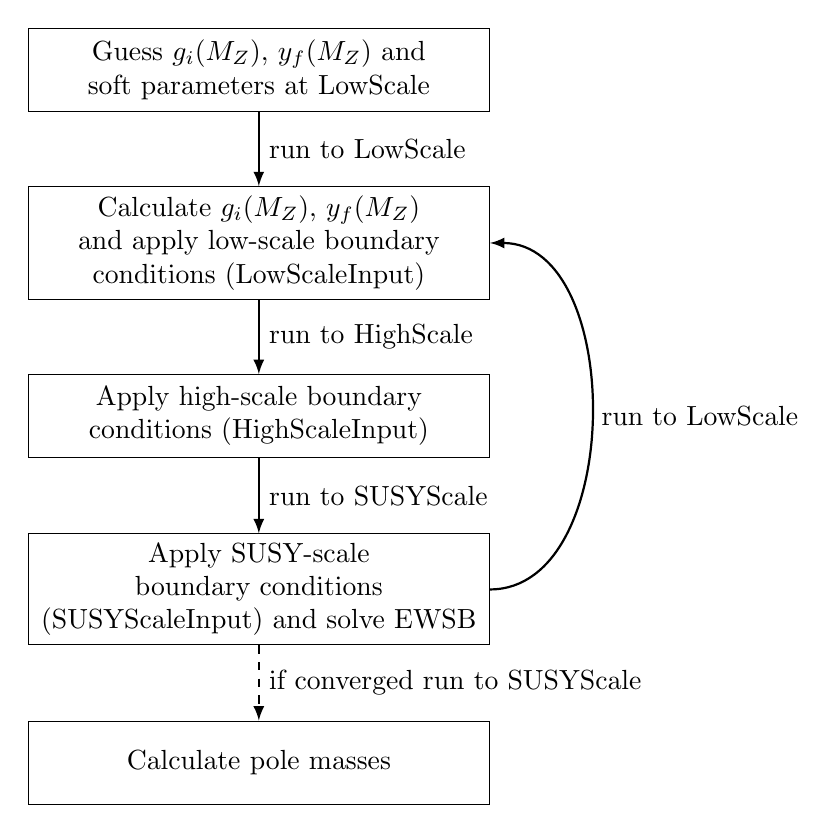
\begin{tikzpicture}[node distance = 2.2cm, auto]
    \tikzstyle{block} = [rectangle, draw, text width=16em, text centered, minimum height=3em]
    \tikzstyle{arrow} = [draw, -latex, thick]
    \node[block] (guess) {Guess $g_i(M_Z)$, $y_f(M_Z)$ and soft
      parameters at \code{LowScale}};
    \node[block,below of=guess] (MZ) {Calculate $g_i(M_Z)$, $y_f(M_Z)$ and apply
      low-scale boundary conditions (\code{LowScaleInput})};
    \path[arrow] (guess) -- node {run to \code{LowScale}} (MZ);
    \node[block,below of=MZ] (MX) {Apply high-scale boundary conditions
      (\code{HighScaleInput})};
    \path[arrow] (MZ) -- node {run to \code{HighScale}} (MX);
    \node[block,below of=MX] (MS) {Apply SUSY-scale boundary conditions
      (\code{SUSYScaleInput}) and solve EWSB};
    \path[arrow] (MX) -- node {run to \code{SUSYScale}} (MS);
    %\path[arrow] (MS.east) -| node {run to \code{LowScale}} (MZ.east);
    \path[-latex, thick] (MS.east) edge[bend right=90] node[right] {run to \code{LowScale}} (MZ.east);
    \node[block,below of=MS] (spec) {Calculate pole masses};
    \path[arrow,dashed] (MS) -- node[text width=16em] {if converged run to \code{SUSYScale}} (spec);
  \end{tikzpicture}
  \caption{Iterative two-scale algorithm to calculate the spectrum.}
  \label{fig:two-scale-algorithm}
\end{figure}

\subsection{Pole masses}
\label{sec:PoleMasses}
After the solver routine has finished and convergence has been
achieved, all \DRbar\ parameters consistent with the EWSB conditions,
low energy data and all user-supplied boundary conditions and are
known at any scale between \code{LowScale} and \code{HighScale}.

The (physical) pole mass spectrum can now be calculated.  \fs uses the
full one-loop self-energies and tree-level mass matrices obtained from
SARAH to calculate the pole masses, which means finding the values $p$
that solve the equation
%
\begin{align}
  0 = \det\left[p^2\unity - m_{f,1L}(p^2)\right].
  \label{eq:pole-mass-def}
\end{align}
%
Here the one-loop mass matrix $m_{f,1L}(p^2)$ for field $f$ is given
in terms of the tree-level mass matrix $m_f$ and the self-energy
$\Sigma_f(p^2)$ as
%
\begin{align}
  &\text{scalars } \phi: &
  m_{\phi,1L}(p^2) &= m_{\phi} - \Sigma_\phi(p^2), \\
  &\text{Majorana fermions } \chi: &
  m_{\chi,1L}(p^2) &= m_{\chi} - \frac{1}{2}\Big[
    \Sigma_\chi^S(p^2) + \Sigma_\chi^{S,T}(p^2)
    + \Big( \Sigma_\chi^{L,T}(p^2) + \Sigma_\chi^R(p^2) \Big) m_{\chi} \notag \\
    &&&\phantom{= m_{\chi} - \frac{1}{2}\Big[}
    + m_{\chi} \Big( \Sigma_\chi^L(p^2) + \Sigma_\chi^{R,T}(p^2) \Big)
  \Big], \\
  &\text{Dirac fermions } \psi: &
  m_{\psi,1L}(p^2) &= m_{\psi}
  - \Sigma_\psi^S(p^2)
  - \Sigma_\psi^R(p^2) m_{\psi}
  - m_{\psi} \Sigma_\psi^L(p^2) .
\end{align}
%
Eq.~\eqref{eq:pole-mass-def} can be solved by diagonalizing the
one-loop mass matrix $m_{f,1L}(p^2)$.  However, since $m_{f,1L}(p^2)$
depends on the momentum $p$, an iteration over $p$ must be performed.
Since this iteration can be very time consuming for large field
multiplets, \fs provides two approximative procedures with a faster
run-time.  The used procedure can be set in the model file for each
field.  These approximations work as follows:
%
\begin{itemize}
\item \code{LowPoleMassPrecision}: This option provides the
  lowest precision but is also the fastest one.  Here the one-loop
  mass matrix $m_{f,1L}^\text{low}$ is calculated exactly once as
%
  \begin{align}
    \forall i,j: (m_{f,1L}^\text{low})_{ij} = (m_{f,1L}(p^2 = m_{f_i}
    m_{f_j}))_{ij} ,
  \end{align}
%
  where $m_{f_i}$ is the $i$th mass eigenvalue of the tree-level mass
  matrix $m_f$.  Afterwards, $m_{f,1L}^\text{low}$ is diagonalized and
  the eigenvalues are interpreted as pole masses $m_{f_i}^\pole$.
  This method neglects which are formally of two-loop order.  This
  method is imprecise if the self-energy corrections to the mass
  matrix are large or the tree-level mass spectrum of the multiplet is
  very split.

\item \code{MediumPoleMassPrecision} (default): This option
  provides calculation with medium precision with a medium execution
  time.  Here the one-loop mass matrix $m_{f,1L}^\text{medium}$ is
  calculated $n$ times as
%
  \begin{align}
    (m_{f,1L}^\text{medium})_{ij}^{(k)} = (m_{f,1L}(p^2 =
    m_{f_k}^2))_{ij} , \qquad k = 1,\ldots,n ,
  \end{align}
%
  where $m_{f_k}$ is the $k$th mass eigenvalue of the tree-level mass
  matrix $m_f$.  Afterwards, each mass matrix
  $(m_{f,1L}^\text{medium})^{(k)}$ is diagonalized and the $k$th
  eigenvalue is interpreted as pole mass $m_{f_k}^\pole$.  This method
  is imprecise if the self-energy corrections to the mass matrix are
  large.

\item \code{HighPoleMassPrecision}: This option solves
  Eq.~\eqref{eq:pole-mass-def} exactly by iterating over the momentum
  $p$.  It therefore provides the determination of the pole masses
  with highest precision, but has also the highest execution time.
  Here the one-loop mass matrix $m_{f,1L}^\text{high}$ is diagonalized
  $n$ times, as in the case of \code{MediumPoleMassPrecision},
  resulting in $n$ pole masses $m_{f_k}^\pole$ ($k = 1,\ldots,n$).
  Afterwards, the diagonalization is repeated, this time using the
  calculated pole masses $m_{f_k}^\pole$ for the momentum calculation
  $p^2 = (m_{f_k}^\pole)^2$.  The iteration stops if convergence is
  reached.
\end{itemize}
%
If higher accuracy is required, two-loop corrections to the
self-energies can be added by setting \code{UseHiggs2LoopMSSM = True}
in the MSSM or \code{UseHiggs2LoopNMSSM = True} in the NMSSM in the
model file.  This enables two-loop Higgs FORTRAN routines supplied by
P.~Slavich from
\cite{Degrassi:2001yf,Brignole:2001jy,Dedes:2002dy,Brignole:2002bz,Dedes:2003km}
which add two-loop corrections of $\oatas$, $\oabas$, $\oatq$,
$\oabq$, $\oatauq$ and $\oatab$.  Something similar is
done for the NMSSM, but in this case the NMSSM $\oatas$, $\oabas$
pieces come from \cite{Degrassi:2009yq}, while for $\oatq$,
$\oabq$, $\oatauq$ and $\oatab$ the MSSM pieces are used
though it should be understood that these are not complete in the
NMSSM. For other models since the Higgs mass is a very important
measurement and the two-loop corrections can be larger than the
current experimental error \cite{Degrassi:2009yq} we recommend that
the leading log two-loop corrections are estimated, by generalizing
those of the MSSM or NMSSM, as has been done, for example, in the
E$_6$SSM \cite{King:2005jy}.

\section{Flexible Applications}
\label{sec:Flexible}

By definition, research is an endeavor to find something new.
Therefore, it can often be the case that
a spectrum generator right out of the box is not enough.
\fs attempts to offer a clean interface through which
one can exploit its facilities
while undergoing a minimal amount of frustration,
when he or she programs for a wide variety of studies.
In what follows,
this property shall be demonstrated by presenting a few use cases
at differing levels of complexity.

To avoid confusion,
it should be mentioned that
the code snippets presented below are not
verbatim listings of the files included in the package.
They have been tailored retaining the semantics
for conciseness.

\subsection{Adapting model files}
\label{sec:adapting-model-files}

There are simple but interesting goals
that one can achieve only by working on
\mathematica files.
The outcome thus obtained from \fs
might already include a fully-fledged program
that is useful in physics analysis.
In a more advanced project,
one might utilize the produced libraries as building blocks
that constitute the target application.
For a general account of the \fs model files,
refer to \secref{sec:modfile}.

\subsubsection{Changing boundary conditions}
\label{sec:changing boundary conditions}

As already emphasized in \secref{sec:Program}, the modular design of
\fs makes it straightforward % to change a boundary condition.
% Within the present C++ code structure,
% this task reduces
to replace a boundary condition object.
The question then becomes how
one could obtain an alternative boundary condition class,
apart from writing one by hand.
The meta code feature of \fs offers great assistance
in this respect.
An example shall be presented to illustrate how this works.

In the literature,
there is a popular alternative to the CMSSM boundary condition
under which the Higgs soft masses are allowed to be different from
the universal mass of the other scalars \cite{NUHM}.
One might implement
this non-universal Higgs-mass MSSM (NUHMSSM) scenario
simply by modifying the model description given to \fs.
A section of the \code{FlexibleSUSY.m.in} file is listed below:
\begin{numlstlisting}
EXTPAR = {{1, mHd2In}, {2, mHu2In}};

HighScaleInput={
  {mHd2, mHd2In}, {mHu2, mHu2In},
  {T[Ye], Azero*Ye}, {T[Yd], Azero*Yd}, {T[Yu], Azero*Yu},
  {mq2, UNITMATRIX[3] m0^2}, {ml2, UNITMATRIX[3] m0^2}, {md2, UNITMATRIX[3] m0^2},
  {mu2, UNITMATRIX[3] m0^2}, {me2, UNITMATRIX[3] m0^2},
  {MassB, m12}, {MassWB, m12}, {MassG, m12}
};
\end{numlstlisting}
Since \code{mHd2} and \code{mHu2} are to be fixed at constants
different from \code{m0^2},
two additional input parameters,
\code{mHd2In} and \code{mHu2In}, holding those constants,
are introduced in the list \code{EXTPAR}.
These input parameters are then declared to be the high-scale values of
\code{mHd2} and \code{mHu2} in line 4.
The rest of the boundary conditions is the same as in the CMSSM\@.
In the SLHA input file,
the parameter indices \code{1} and \code{2} of
\code{mHd2In} and \code{mHu2In}, declared in \code{EXTPAR} above,
must appear
as the first field in each line in the \code{EXTPAR} block:
\begin{numlstlisting}
Block EXTPAR
    1   10000                # mHd2In
    2   -2500                # mHu2In
\end{numlstlisting}
Note that the two additional input parameters are chosen to have
mass dimension 2, unlike \code{m0}.
This makes it easy to
try both signs of the high-scale value of either soft Higgs mass squared,
as exemplified in line 3.
If one were not interested in a negative boundary value of \code{mHu2}
for instance,
then a dimension-1 parameter %, \code{mHuIn},
might instead be introduced whose square is equated with \code{mHu2}.

The full implementation is available
in \code{model_files/NUHMSSM/}.
To try it out, do the following:
\begin{numlstlisting}[language=bash]
$ ./createmodel --name=NUHMSSM --sarah-model=MSSM
$ ./configure --with-models=NUHMSSM
$ make
$ models/NUHMSSM/run_NUHMSSM.x --slha-input-file=model_files/NUHMSSM/LesHouches.in.NUHMSSM
\end{numlstlisting}
Notice the \code{--sarah-model=MSSM} flag in line 1.
It tells the \code{createmodel} script to reuse
the MSSM specification in \sarah
to generate the C++ program.

\subsubsection{Extending existing models}

The preceding example was a modest alteration of a physics scenario
in that an existing model has been reused.
A more non-trivial modification might involve
an extension of the particle content as well as the interactions.
One of the simplest classes of models beyond the MSSM is
those with additional gauge-single fields.
In what follows, a supersymmetric type-I see-saw model
\cite{see-saw}
shall be considered in which
three neutral (heavy) chiral superfields are introduced.

% To create a new model, one should name it.
In the package, this model is named \code{MSSMRHN}, standing for
the MSSM plus right-handed neutrinos.
% Since \fs needs the outcome of \sarah,
One needs to prepare an input file to \sarah which might be placed in
\code{<FlexibleSUSY-root>/sarah/MSSMRHN/} or
\code{<SARAH-root>/Models/MSSMRHN/}.
The input file \code{MSSMRHN.m} contains
the declaration of the three-generation singlets \code{v}:
\begin{numlstlisting}[name=MSSMRHN.m]
SuperFields[[8]] = {v, 3, conj[vR], 0, 1, 1, RpM};
\end{numlstlisting}
as well as the neutrino Yukawa couplings and the Majorana mass terms
of the singlets:
\begin{numlstlisting}[name=MSSMRHN.m]
SuperPotential = Yu u.q.Hu - Yd d.q.Hd - Ye e.l.Hd + \[Mu] Hu.Hd +
                 Yv v.l.Hu + Mv/2 v.v;
\end{numlstlisting}
Further declarations inform \sarah
of how to form Dirac spinors out of the new Weyl spinors
and how the scalars and the fermions mix to comprise
the mass eigenstates:
\begin{numlstlisting}[name=MSSMRHN.m]
DEFINITION[GaugeES][DiracSpinors] = {
  Fu1 -> {FuL, 0}, Fu2 -> {0, FuR},
  Fv1 -> {FvL, 0}, Fv2 -> {0, FvR},
  ...
};

DEFINITION[EWSB][MatterSector] = {
  {{SuL, SuR}, {Su, ZU}},
  {{SvL, SvR}, {Sv, ZV}},
  ...
  {{fB, fW0, FHd0, FHu0}, {L0, ZN}},
  {{FvL, conj[FvR]}, {FV, UV}},
  {{{fWm, FHdm}, {fWp, FHup}}, {{Lm, UM}, {Lp, UP}}},
  {{{FuL}, {conj[FuR]}}, {{FUL, ZUL}, {FUR, ZUR}}}
};

DEFINITION[EWSB][DiracSpinors] = {
  Fu  -> {FUL, conj[FUR]},
  Fv  -> {FV , conj[FV] },
  Chi -> {L0 , conj[L0] },
  Cha -> {Lm , conj[Lp] },
  ...
};
\end{numlstlisting}
With respect to the MSSM file, newly added lines are
6, 12, 15, and 22.
Notice that the (left- and right-handed) neutrino mixing
in line 15 resembles the neutralino mixing in line 14.
Due to the Majorana mass term in the superpotential,
the six neutrino mass eigenstates are described in terms of
Majorana spinors like the neutralinos.

One should then add descriptions of the new states in the file
\code{particles.m}:
\begin{numlstlisting}
ParticleDefinitions[GaugeES] = {
  {Fv1, { Description -> "Dirac Left Neutrino" }},
  {Fv2, { Description -> "Dirac Right Neutrino" }},
  {SvR, { Description -> "Right Sneutrino", LaTeX ->"\\tilde{\\nu}_R"}},
  ...
};

ParticleDefinitions[EWSB] = {
  {Sv, { Description -> "Sneutrinos",
         PDG -> {1000012, 1000014, 1000016, 2000012, 2000014, 2000016}}},
  {Fv, { Description -> "Neutrinos",
         PDG -> {12, 14, 16, 9900012, 9900014, 9900016}}},
  ...
};

WeylFermionAndIndermediate = {
  {v,   { Description -> "Right Neutrino Superfield" }},
  {FV,  { Description -> "Neutrino-Masseigenstate"}},
  {FvL, { Description -> "Left Neutrino"}},
  {FvR, { Description -> "Right Neutrino"}},
  ...
};
\end{numlstlisting}
In line 12, one finds PDG codes beginning with \code{99}.
Such numbers are available for a program author's private use
\cite{Beringer:1900zz}.
The new parameters in the superpotential
and the soft supersymmetry breaking sector
are to be described in \code{parameters.m}:
\begin{numlstlisting}
ParameterDefinitions = {
  {UV,    { Description -> "Neutrino-Mixing-Matrix"}},
  {Yv,    { Description -> "Neutrino-Yukawa-Coupling" }},
  {T[Yv], { Description -> "Trilinear-Neutrino-Coupling"}},
  {Mv,    { LaTeX -> "M_v", OutputName -> Mv, LesHouches -> Mv}},
  {B[Mv], { LaTeX -> "B_v", OutputName -> BMv, LesHouches -> BMv}},
  {mv2,   { Description -> "Softbreaking right Sneutrino Mass"}},
  ...
};
\end{numlstlisting}
For details on how to write model files for \sarah, consult its manual.

Finally, it remains to put \code{FlexibleSUSY.m.in}
in \code{model_files/MSSMRHN/}.
The high-scale boundary conditions therein might read:
\begin{numlstlisting}
HighScaleInput = {
  {Mv, LHInput[Mv]}, {B[Mv], LHInput[B[Mv]]},
  {Yv, LHInput[Yv]}, {T[Yv], Azero*Yv},
  {mv2, UNITMATRIX[3] m0^2},
  ...
};
\end{numlstlisting}
In this particular example,
the new parameters shown in lines 2--3
are constrained at the $M_X$ scale
to the values given in the SLHA input file.
In a data-driven approach,
they might alternatively be fixed from a matching against
a low-energy theory containing the dimension-5
neutrino mass operator in conjunction with supplementary constraints.

With the above set of input files,
\fs can generate the C++ code and compile it
to produce \code{libMSSMRHN}.
These products shall be employed as the implementation of the theory that
underlies the MSSM in the next subsection.

\subsection{Adapting C++ code}
\label{sec:adapting-cpp-code}

There are problems which one cannot solve only by
editing \mathematica model files.
To unlock the full potential of \fs,
it is an advantage not to avoid programming at the C++ level.
For this, it should help to have working knowledge about the basic structure
of a spectrum generator, set out in \secref{sec:SpecGenStruct}.
In what follows,
it shall be demonstrated that
the clean object structure serves as firm guidance on the job.

\subsubsection{Stacking models in a tower of effective theories}
\label{sec:tower construction}

Consider a physics scenario which is best described
by a tower of effective theories.
Within the framework of \fs, the C++ object structure is
a faithful reflection of
this physicist's view on the given problem.
This point might be illustrated
using a well-known configuration in which
the higher-energy theory is the MSSMRHN discussed above which
gives rise to the MSSM as the lower-energy effective theory.
The relevant objects are sketched
in \figref{fig:class structure for tower}.
\begin{figure}
  \centering
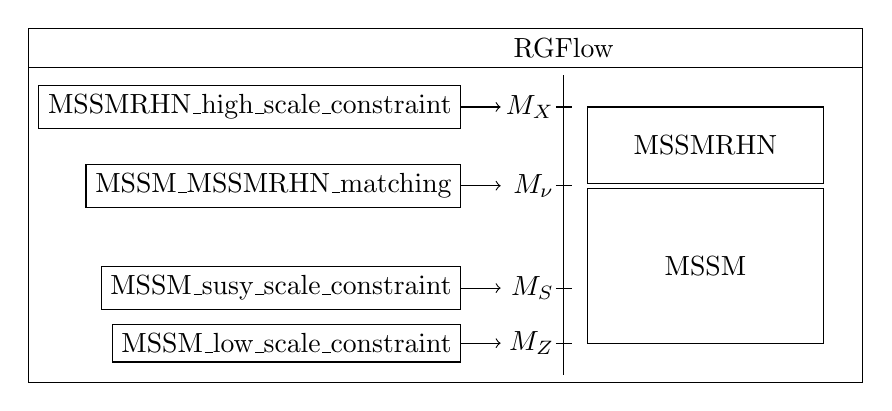
\begin{tikzpicture}
  \draw (0,-.5) coordinate(bottom)
        (0,-.4)
     -- (0,0)  coordinate(MZ) node[left] {$M_Z$}
     -- (0,.7) coordinate(MS) node[left] {$M_S$}
     -- (0,2)  coordinate(Mv) node[left] {$M_\nu$}
     -- (0,3)  coordinate(MX) node[left] {$M_X$}
     -- (0,3.4)
        (0,3.5) coordinate(top);

  \path (MZ) ++(.3,0) coordinate(MZR) +(3,0) coordinate(MZRR)
        (MS) ++(.3,0) coordinate(MSR) +(3,0) coordinate(MSRR)
        (Mv) ++(.3,0) coordinate(MvR) +(3,0) coordinate(MvRR)
        (MX) ++(.3,0) coordinate(MXR) +(3,0) coordinate(MXRR);

  \draw (MZ) +(-.1,0) -- +(+.1,0); \draw[<-] (MZ) ++(-.8,0) -- ++(-.5,0)
     node[left,draw] {\code{MSSM_low_scale_constraint}};
  \draw (MS) +(-.1,0) -- +(+.1,0); \draw[<-] (MS) ++(-.8,0) -- ++(-.5,0)
     node[left,draw] {\code{MSSM_susy_scale_constraint}};
  \draw (Mv) +(-.1,0) -- +(+.1,0); \draw[<-] (Mv) ++(-.8,0) -- ++(-.5,0)
     node[left,draw] {\code{MSSM_MSSMRHN_matching}};
  \draw (MX) +(-.1,0) -- +(+.1,0); \draw[<-] (MX) ++(-.8,0) -- ++(-.5,0)
     node[left,draw] {\code{MSSMRHN_high_scale_constraint}};

  \draw (MvRR) +(0,-.03) rectangle (MZR) node[pos=.5] {\code{MSSM}};
  \draw (MvRR) +(0, .03) rectangle (MXR) node[pos=.5] {\code{MSSMRHN}};

  \path (bottom) +(3.8,0) coordinate(SE) (top) +(-6.8,0) coordinate(NW);
  \draw  (NW) +(0,.5) rectangle (SE)
         (NW) -- +(10.6,0);
  \path (top) node[above] {\code{RGFlow}};
\end{tikzpicture}
  \caption{Schematic object structure in the C++ code for
    the tower scenario.}
  \label{fig:class structure for tower}
\end{figure}
The \code{MSSMRHN} object is in effect from the $M_X$ scale down to
the $M_\nu$ scale at which the right-handed neutrinos are decoupled.
Below this scale, the \code{MSSM} object takes over.
On the left of the vertical axis,
the boundary condition objects acting on either model are displayed,
together with the matching object connecting the two theories.
Note that each of the boundary condition and matching objects
maintains and updates its own scale over iterations.
An arrow in the figure depicts
the association of a constraint with its scale.
All these components are plugged into the \code{RGFlow} object
which then solves the problem.

Since the current implementation of \fs does not (yet)
produce a spectrum generator spanning multiple models,
one needs to write the matching object
% in \figref{fig:class structure for tower}
as well as gluing codes by hand to build such a program.
One can author nearly all the components of a multi-model spectrum generator
by making a straightforward extension
to each corresponding single-model counterpart
for one of the models forming the tower.
Obviously, this tip does not work for the matching class,
which has no analogue in a single-model case.

As the target spectrum generator depends on two models,
one should first build these prerequisites by:
\begin{numlstlisting}
$ ./createmodel --name=MSSM
$ ./createmodel --name=MSSMRHN
$ ./configure --with-models=MSSM,MSSMRHN
$ make
\end{numlstlisting}
As a by-product, line 3
also creates a \code{Makefile} in \code{examples/tower/}.
One could best see the overall code structure of the application in this file:
\begin{numlstlisting}
CPPFLAGS  := -I. $(INCCONFIG) $(INCFLEXI) $(INCLEGACY) $(INCSLHAEA) \
             $(INCMSSM) $(INCMSSMRHN)

TOWER_SRC := run_tower.cpp \
	     MSSM_MSSMRHN_two_scale_matching.cpp \
	     MSSM_MSSMRHN_two_scale_initial_guesser.cpp

TOWER_OBJ := $(patsubst %.cpp, %.o, $(filter %.cpp, $(TOWER_SRC)))

run_tower.x: $(TOWER_OBJ) $(LIBMSSM) $(LIBMSSMRHN) $(LIBFLEXI) $(LIBLEGACY)
  $(CXX) -o $@ $^ $(LOOPFUNCLIBS) $(GSLLIBS) $(BOOSTTHREADLIBS) $(THREADLIBS) $(LAPACKLIBS) $(FLIBS)
\end{numlstlisting}
This file is created in \code{examples/tower/}
on the execution of the \code{configure} script.
The include directives in line 2 tell the compiler
where to find the headers for either \code{MSSM} or \code{MSSMRHN}.
The \code{.cpp} files in lines 4--6 and the \code{.hpp} files
that they include are to be written by hand.
Obviously, the executable \code{run_tower.x}, in line 10, depends on both
\code{$(LIBMSSM)} and \code{$(LIBMSSMRHN)}
that implement the auto-generated
components in \figref{fig:class structure for tower}.

To prepare the main source file \code{run_tower.cpp},
one can extend % make a straightforward extension to
\code{run_MSSM.cpp} or \code{run_MSSMRHN.cpp}
produced in either model directory.
The shipped example reads:
\begin{numlstlisting}
#include "MSSM_MSSMRHN_spectrum_generator.hpp"

int main(int argc, char* argv[])
{
  // define objects;
  QedQcd oneset;
  MSSM_input_parameters    input_1;
  MSSMRHN_input_parameters input_2;
  // fill in input_1 and input_2;
  oneset.toMz(); // run SM fermion masses to MZ
  typedef Two_scale algorithm_type;
  MSSM_MSSMRHN_spectrum_generator<algorithm_type> spectrum_generator;
  // set up spectrum_generator;
  spectrum_generator.run(oneset, input_1, input_2);
  // extract outcome from models;
}
\end{numlstlisting}
where a line in the form \code{// ...;} shall be understood
to be a pseudo-code.
Given two models,
one declares two sets of input parameters,
\code{input_1} and \code{input_2}, in lines 7--8.
The suffixes \code{_1} and \code{_2} are not necessary but intended to remind
the programmer of to which model the object is relevant.

The \code{main} function then delegates
the \code{MSSM_MSSMRHN_spectrum_generator} object
to set up and drive the \code{RGFlow} object in
\figref{fig:class structure for tower}.
This task is started by the call in line 14 to
the following member function defined in
\code{MSSM_MSSMRHN_spectrum_generator.hpp}:
\begin{numlstlisting}[name=SGrun]
template<class T> void MSSM_MSSMRHN_spectrum_generator<T>::run
(const QedQcd& oneset,
 const MSSM_input_parameters& input_1, const MSSMRHN_input_parameters& input_2)
{
  high_scale_constraint_2.clear(); // of type MSSMRHN_high_scale_constraint<T>
  susy_scale_constraint_1.clear(); // of type MSSM_susy_scale_constraint<T>
  low_scale_constraint_1 .clear(); // of type MSSM_low_scale_constraint<T>
  matching.reset();                // of type MSSM_MSSMRHN_matching<T>
  high_scale_constraint_2.set_input_parameters(input_2);
  susy_scale_constraint_1.set_input_parameters(input_1);
  low_scale_constraint_1 .set_input_parameters(input_1);
  matching.set_upper_input_parameters(input_2);
  high_scale_constraint_2.initialize();
  susy_scale_constraint_1.initialize();
  low_scale_constraint_1 .initialize();
  if (!is_zero(input_scale_2)) high_scale_constraint_2.set_scale(input_scale_2);
\end{numlstlisting}
This piece of code is nearly a verbatim copy of
the corresponding part of \code{MSSM_spectrum_generator.hpp}.
The only differences are that the type of
\code{high_scale_constraint_2} is
\code{MSSMRHN_high_scale_constraint<T>} and that
the \code{matching} object has been added.
Recall that the template parameter \code{T} has been bound to
\code{Two_scale} in the \code{main} function.
One then constructs a list of
the constraints on \code{MSSM}:
\begin{numlstlisting}[name=SGrun]
  std::vector<Constraint<T>*> upward_constraints_1;
  upward_constraints_1.push_back(&low_scale_constraint_1);
  std::vector<Constraint<T>*> downward_constraints_1;
  downward_constraints_1.push_back(&susy_scale_constraint_1);
  downward_constraints_1.push_back(&low_scale_constraint_1);
\end{numlstlisting}
and initializes the \code{MSSM} object:
\begin{numlstlisting}[name=SGrun]
  model_1.clear();                 // of type MSSM<T>
  model_1.set_input_parameters(input_1);
  model_1.do_calculate_sm_pole_masses(calculate_sm_masses);
\end{numlstlisting}
Likewise for \code{MSSMRHN}:
\begin{numlstlisting}[name=SGrun]
  std::vector<Constraint<T>*> upward_constraints_2;
  upward_constraints_2.push_back(&high_scale_constraint_2);
  std::vector<Constraint<T>*> downward_constraints_2;
  downward_constraints_2.push_back(&high_scale_constraint_2);
  model_2.clear();                 // of type MSSMRHN<T>
  model_2.set_input_parameters(input_2);
\end{numlstlisting}
Note that \code{model_2} does not have to calculate the pole masses of
the SM particles since it is active only above $M_\nu$
which is assumed to be much higher than the weak scale.
To test the convergence of both models,
one may construct a composite convergence tester
out of auto-generated
\code{MSSM_convergence_tester} and \code{MSSMRHN_convergence_tester}:
\begin{numlstlisting}[name=SGrun]
  MSSM_convergence_tester<T> convergence_tester_1(&model_1, precision_goal);
  MSSMRHN_convergence_tester<T> convergence_tester_2(&model_2, precision_goal);
  if (max_iterations > 0) {
    convergence_tester_1.set_max_iterations(max_iterations);
    convergence_tester_2.set_max_iterations(max_iterations);
  }
  Composite_convergence_tester<T> convergence_tester;
  convergence_tester.add_convergence_tester(&convergence_tester_1);
  convergence_tester.add_convergence_tester(&convergence_tester_2);
\end{numlstlisting}
On construction,
the initial guesser accepts the following parameters
including the two model objects:
\begin{numlstlisting}[name=SGrun]
  MSSM_MSSMRHN_initial_guesser<T> initial_guesser
    (&model_1, &model_2, input_2, oneset,
     low_scale_constraint_1, susy_scale_constraint_1, high_scale_constraint_2,
     matching);
\end{numlstlisting}
The code of the above class shall be presented later on.
One then passes
\code{convergence_tester} and \code{initial_guesser}
to \code{solver}, the \code{RGFlow} object,
along with the precision specification:
\begin{numlstlisting}[name=SGrun]
  Two_scale_increasing_precision precision(10.0, precision_goal);
  solver.reset();                  // of type RGFlow<T>
  solver.set_convergence_tester(&convergence_tester);
  solver.set_running_precision(&precision);
  solver.set_initial_guesser(&initial_guesser);
\end{numlstlisting}
Finally,
one is ready to construct the tower of effective theories
by adding to \code{solver}
each model plus the associated list of constraints
optionally accompanied by a matching object:
\begin{numlstlisting}[name=SGrun]
  solver.add_model(&model_1, &matching, upward_constraints_1, downward_constraints_1);
  solver.add_model(&model_2, upward_constraints_2, downward_constraints_2);
\end{numlstlisting}
The order of addition is from the lowest scale to the highest.
Notice in line 49
that the matching object between \code{model_1} and
\code{model_2} is given when one adds the former, i.e.\ the lower-energy model.
It then remains to solve the boundary value problem:
\begin{numlstlisting}[name=SGrun]
  high_scale_2 = susy_scale_1 = low_scale_1 = 0; matching_scale = 0;
  solver.solve();
\end{numlstlisting}
After the solution is found,
one can obtain the resulting low-energy spectrum.
Since \code{model_1} is in contact with the lowest energy,
let it calculate the spectrum:
\begin{numlstlisting}[name=SGrun]
  susy_scale_1 = susy_scale_constraint_1.get_scale();
  model_1.run_to(susy_scale_1);    // of type MSSM<T>
  model_1.calculate_spectrum();
  if (!is_zero(parameter_output_scale_1))
    model_1.run_to(parameter_output_scale_1);
}
\end{numlstlisting}
In lines 56--57,
the scale is optionally brought to the value at which
one wishes to get the \DRbar\ parameters.

One needs to write the matching class for a particular pair of
models from scratch.
It shall be based on the abstract class \code{Matching<Two_scale>}
that comes with \fs.
In the present example, the class is declared in the header
\code{MSSM_MSSMRHN_two_scale_matching.hpp}:
\begin{numlstlisting}
template<> class MSSM_MSSMRHN_matching<Two_scale> : public Matching<Two_scale> {
public:
  MSSM_MSSMRHN_matching();
  MSSM_MSSMRHN_matching(const MSSMRHN_input_parameters&);
  void match_low_to_high_scale_model();
  void match_high_to_low_scale_model();
  double get_scale() const;
  void set_models(Two_scale_model *lower, Two_scale_model *upper);
  double get_initial_scale_guess() const;
  void set_upper_input_parameters(const MSSMRHN_input_parameters&);
  void set_scale(double);
  void reset();
private:
  MSSM   <Two_scale> *lower;
  MSSMRHN<Two_scale> *upper;
  void make_initial_scale_guess();
  void update_scale();
  ...
};
\end{numlstlisting}
As lines 4 and 10 indicate,
this class takes an \code{MSSMRHN_input_parameters} object as input.
The \code{MvInput} field thereof is referenced
for the initial guess of the matching scale
in line 25 of \code{MSSM_MSSMRHN_two_scale_matching.cpp}:
\begin{numlstlisting}
void MSSM_MSSMRHN_matching<Two_scale>::match_low_to_high_scale_model()
{
  upper->set_Yd(lower->get_Yd());
  // copy rest of couplings from lower to upper;
  upper->set_scale(lower->get_scale());
}

void MSSM_MSSMRHN_matching<Two_scale>::match_high_to_low_scale_model()
{
  update_scale();
  lower->set_Yd(upper->get_Yd());
  // copy rest of couplings from upper to lower;
  lower->set_scale(upper->get_scale());
}

void MSSM_MSSMRHN_matching<Two_scale>::set_upper_input_parameters
(const MSSMRHN_input_parameters& inputPars_)
{
  inputPars = inputPars_;
  make_initial_scale_guess();
}

void MSSM_MSSMRHN_matching<Two_scale>::make_initial_scale_guess()
{
  double RHN_scale = pow(abs(inputPars.MvInput.determinant()), 1.0/3);
  scale = initial_scale_guess = RHN_scale;
}

void MSSM_MSSMRHN_matching<Two_scale>::update_scale()
{
  double RHN_scale = pow(abs(upper->get_Mv().determinant()), 1.0/3);
  scale = RHN_scale;
}
\end{numlstlisting}
Recall that \code{MvInput} is the high-scale boundary value of \code{Mv}.
If one had opted for an alternative strategy to fix \code{Mv},
then \code{MSSM_MSSMRHN_matching} might have required a different input.
Subsequently, the matching scale is updated at each iteration
to be the geometric mean of the running \code{Mv} eigenvalues
in lines 31--32.
The actual matching process takes place in the two functions
\code{match_low_to_high_scale_model} and \code{match_high_to_low_scale_model}.
For brevity,
their examples shown above simply copy each coupling
upwards or downwards, neglecting threshold corrections.
The way to incorporate these corrections should be self-evident
from the code structure.

% \begin{numlstlisting}
% template<>
% class MSSM_MSSMRHN_initial_guesser<Two_scale> : public Initial_guesser<Two_scale> {
% public:
%   MSSM_MSSMRHN_initial_guesser(MSSM<Two_scale>*, MSSMRHN<Two_scale>*,
%                                const MSSMRHN_input_parameters&,
%                                const QedQcd&,
%                                const MSSM_low_scale_constraint<Two_scale>&,
%                                const MSSM_susy_scale_constraint<Two_scale>&,
%                                const MSSMRHN_high_scale_constraint<Two_scale>&,
%                                const MSSM_MSSMRHN_matching<Two_scale>&);
%   virtual ~MSSM_MSSMRHN_initial_guesser();
%   virtual void guess();
%
% private:
%   MSSM   <Two_scale>* model_1;
%   MSSMRHN<Two_scale>* model_2;
%   MSSMRHN_input_parameters input_pars;
%   QedQcd oneset;
%   MSSM_low_scale_constraint<Two_scale> low_constraint;
%   MSSM_susy_scale_constraint<Two_scale> susy_constraint;
%   MSSMRHN_high_scale_constraint<Two_scale> high_constraint;
%   MSSM_MSSMRHN_matching<Two_scale> matching;
% };
% \end{numlstlisting}
The last missing piece is the initial guesser.
One can extend the already available
\code{MSSM_initial_guesser} class. % in a straightforward manner.
The essential task is done by the following member function:
\begin{numlstlisting}[name=MSSM_MSSMRHN_two_scale_initial_guesser.cpp]
void MSSM_MSSMRHN_initial_guesser<Two_scale>::guess()
{
  // guess SUSY couplings in model-1 at low energy;

  const double low_scale_guess_1 = low_constraint_1.get_initial_scale_guess();
  const double high_scale_guess_2 = high_constraint_2.get_initial_scale_guess();
  const double matching_scale_guess = matching.get_initial_scale_guess();
\end{numlstlisting}
Compared to the MSSM case,
the differences are that
the type of \code{high_constraint_2}
is \code{MSSMRHN_high_scale_constraint<Two_scale>} and that
\code{matching_scale_guess} has been inserted.
Due to this intermediate scale,
the initial run-up is divided into two steps,
with a matching procedure in-between:
\begin{numlstlisting}[name=MSSM_MSSMRHN_two_scale_initial_guesser.cpp]
  model_1->run_to(matching_scale_guess); // of type MSSM<Two_scale>
  matching.set_models(model_1, model_2);
  matching.match_low_to_high_scale_model();
  model_2->run_to(high_scale_guess_2);   // of type MSSMRHN<Two_scale>
\end{numlstlisting}
The high-scale constraints are applied to \code{model_2},
the higher-energy model,
and the remaining undetermined parameters are guessed:
\begin{numlstlisting}[name=MSSM_MSSMRHN_two_scale_initial_guesser.cpp]
  high_constraint_2.set_model(model_2);
  high_constraint_2.apply();
  model_2->set_Mu(1.0); model_2->set_BMu(0.0);
\end{numlstlisting}
The initial two-step run-down again involves a matching process:
\begin{numlstlisting}[name=MSSM_MSSMRHN_two_scale_initial_guesser.cpp]
  model_2->run_to(matching_scale_guess);
  matching.match_high_to_low_scale_model();
  model_1->run_to(low_scale_guess_1);
\end{numlstlisting}
At the low scale where \code{MSSM} is valid,
the code is the same as in \code{MSSM_initial_guesser}:
\begin{numlstlisting}[name=MSSM_MSSMRHN_two_scale_initial_guesser.cpp]
  model_1->solve_ewsb_tree_level();
  model_1->calculate_DRbar_parameters();
  model_1->set_thresholds(3); model_1->set_loops(2);
}
\end{numlstlisting}

Finally,
one prescribes the additional input parameters in the SLHA input file:
\begin{numlstlisting}
Block YvIN                   # neutrino Yukawas at MX
1 1  0.1568611               # Yv(1,1)
1 2  0.6400513               # Yv(1,2)
1 3  0.7521494               # Yv(1,3)
2 1  0.4663838               # Yv(2,1)
...                          # remaining 5 entries
Block MvIN                   # heavy neutrino masses at MX
1 1  4.150000E+14            # Mv(1,1)
...                          # remaining 8 entries
Block BMvIN                  # right-handed sneutrino bilinear terms
1 1  1.000000E+02            # BMv(1,1)
...                          # remaining 8 entries
\end{numlstlisting}
The file in the package contains the values that approximately reproduce
the observed neutrino masses and mixing angles
\cite{Beringer:1900zz}
through the see-saw mechanism.

For further details, browse the directory \code{examples/tower/}.
One can build and run the example therein by:
\begin{numlstlisting}
$ cd examples/tower
$ make
$ ./run_tower.x --slha-input-file=LesHouches.in.tower
\end{numlstlisting}%% $
In the output,
a part of significant physical interest might be:
\begin{numlstlisting}
Block MSL2 Q=   8.97114431E+02
  1  1     1.25652698E+05   # ml2(1,1)
  1  2    -7.64196328E+01   # ml2(1,2)
  1  3    -7.08429254E+01   # ml2(1,3)
  2  1    -7.64196328E+01   # ml2(2,1)
  2  2     1.25388732E+05   # ml2(2,2)
  2  3    -3.15865242E+02   # ml2(2,3)
  3  1    -7.08429254E+01   # ml2(3,1)
  3  2    -3.15865242E+02   # ml2(3,2)
  3  3     1.24556532E+05   # ml2(3,3)
\end{numlstlisting}
This result demonstrates the well-known effect on
the off-diagonal slepton mass matrix elements
from a non-trivial flavour structure of \code{Yv}
\cite{Borzumati:1986qx}.
This leads in turn to the slepton mixing
matrices, \code{ZE} and \code{ZV},
which contain intergenerational mixings apart from the
generic left-right mixings.

\subsubsection{Integrating custom-built C++ components}
\label{sec:integrating-custom-built}

In \secref{sec:changing boundary conditions},
it was explained how one can let \fs generate
an alternative boundary condition class
by authoring a model file.
Nonetheless, the way to employ this class at the C++ level
might still remain obscure to the reader
since \fs automatically took care of it.
Here, an example shall be exhibited
with the emphasis on the modular C++ code structure
that helps programming.
Concretely,
the auto-generated low-energy boundary condition on the MSSM
shall be modified so that
$\alpha_{\text{s},\text{susy}}^{\text{\DRbar}}$
is determined from
$\alpha_{\text{s},\text{SM}}^{(5),\text{\MSbar}}$
by means of a two-loop matching.
This shall be accompanied by an improvement
of the $g_3$ $\beta$-function to the three-loop accuracy.

The first step is to alter
the model class which evaluates the $\beta$-functions.
Thanks to the \code{beta()} method being virtual,
one can override it conveniently by deriving a class from \code{MSSM}.
The declaration might look like:
% MSSMcbs_two_scale_model.hpp
\begin{numlstlisting}
#include "MSSM_two_scale_model.hpp"

template<>
class MSSMcbs<Two_scale> : public MSSM<Two_scale> {
public:
  explicit MSSMcbs(const MSSM_input_parameters& input_ = MSSM_input_parameters());
  virtual ~MSSMcbs();
  virtual Eigen::ArrayXd beta() const;
  MSSM_soft_parameters calc_beta() const;
};
\end{numlstlisting}
where the name \code{MSSMcbs} is an abbreviation of
the MSSM with custom-built $\beta$'s.
Note that the objects for \code{MSSM} are reused where possible:
\code{MSSM_input_parameters} in line 6 as well as
\code{MSSM_soft_parameters} in line 9.
This saves the programmer from excessive duplication of codes.
The member function definitions read:
\begin{numlstlisting}
Eigen::ArrayXd MSSMcbs<Two_scale>::beta() const
{
  return calc_beta().get();
}

MSSM_soft_parameters MSSMcbs<Two_scale>::calc_beta() const
{
  MSSM_soft_parameters betas(MSSM<Two_scale>::calc_beta());
  if (get_loops() <= 2) return betas;
  double bg33 = /* formula in terms of g1, g2, g3, Yu, Yd, Ye */;
  betas.set_g3(betas.get_g3() + Power(oneOver16PiSqr,3) * g3 * bg33);
  return betas;
}
\end{numlstlisting}
The full C++ expression of \code{bg33},
used in \code{MSSMcbs_two_scale_model.cpp},
has been adapted from the code by Jack and Jones \cite{3-loop MSSM betas}.
This already completes the amendment of the $g_3$ $\beta$-function.

The next step is to write a substitute for
the low-energy boundary condition class.
It must be declared as a descendent of \code{Constraint<Two_scale>}:
% MSSMcbs_two_scale_low_scale_constraint.hpp
\begin{numlstlisting}
#include "two_scale_constraint.hpp"

template<>
class MSSMcbs_low_scale_constraint<Two_scale> : public Constraint<Two_scale> {
public:
  MSSMcbs_low_scale_constraint(const MSSM_input_parameters&, const QedQcd&);
  virtual ~MSSMcbs_low_scale_constraint();
  void set_threshold_corrections(unsigned);
  ...
private:
  MSSMcbs<Two_scale>* model;
  QedQcd oneset;
  double new_g3;
  unsigned threshold_corrections;
  void calculate_DRbar_gauge_couplings();
  double calculate_alS5DRbar_over_alS5MSbar(double) const;
  double calculate_zeta_g_QCD_2(double) const;
  double calculate_zeta_g_SUSY_2(double) const;
  ...
};
\end{numlstlisting}
In line 11,
the type of \code{model} has been adapted to the new model.
In fact, this class should work even if \code{model} remained
a pointer to \code{MSSM<Two_scale>} because of inheritance.
The main additions to \code{MSSM_low_scale_constraint}
in \code{models/MSSM/} are the member functions in lines 16--18,
which evaluate the two-loop matching coefficients
from Ref.~\cite{Harlander:2005wm}.
The following member function then performs
the two-step decoupling as reported in this reference:
% MSSMcbs_two_scale_low_scale_constraint.cpp
\begin{numlstlisting}
void MSSMcbs_low_scale_constraint<Two_scale>::calculate_DRbar_gauge_couplings()
{
  ...
  double alpha_s = oneset.displayAlpha(ALPHAS);
  double alS5DRbar_over_alS5MSbar = 1;
  double zeta_g_QCD_2 = 1;
  double zeta_g_SUSY_2 = 1;
  if (model->get_thresholds()) {
    alS5DRbar_over_alS5MSbar = calculate_alS5DRbar_over_alS5MSbar(alpha_s);
    alpha_s *= alS5DRbar_over_alS5MSbar;  // alS5MSbar -> alS5DRbar
    zeta_g_QCD_2 = calculate_zeta_g_QCD_2(alpha_s);
    alpha_s /= zeta_g_QCD_2;		  // alS5DRbar -> alS6DRbar
    zeta_g_SUSY_2 = calculate_zeta_g_SUSY_2(alpha_s);
    alpha_s /= zeta_g_SUSY_2;		  // alS6DRbar -> alS6DRbarMSSM
    ...
  }
  new_g3 = Sqrt(4*Pi * alpha_s);
  ...
}
\end{numlstlisting}
Finally,
one can integrate the new boundary condition class
\code{MSSMcbs_low_scale_constraint} together with
the new model \code{MSSMcbs}
into the spectrum generator in a straightforward manner.
They should supersede
\code{MSSM_low_scale_constraint} and \code{MSSM}, respectively.
The replacement should be carried out in
those objects that depend on these classes,
i.e.\ the initial guesser:
\begin{numlstlisting}
template<>
class MSSMcbs_initial_guesser<Two_scale> : public Initial_guesser<Two_scale> {
public:
  MSSMcbs_initial_guesser(MSSMcbs<Two_scale>*,
                          const MSSM_input_parameters&,
                          const QedQcd&,
                          const MSSMcbs_low_scale_constraint<Two_scale>&,
                          const MSSM_susy_scale_constraint<Two_scale>&,
                          const MSSM_high_scale_constraint<Two_scale>&);
  ...
private:
  MSSMcbs<Two_scale>* model;
  MSSM_input_parameters input_pars;
  QedQcd oneset;
  MSSMcbs_low_scale_constraint<Two_scale> low_constraint;
  MSSM_susy_scale_constraint<Two_scale> susy_constraint;
  MSSM_high_scale_constraint<Two_scale> high_constraint;
  ...
};
\end{numlstlisting}
as well as the spectrum generator object:
% MSSMcbs_spectrum_generator.hpp
\begin{numlstlisting}
template <class T>
void MSSMcbs_spectrum_generator<T>::run(const QedQcd& oneset,
					const MSSM_input_parameters& input)
{
  ...
  MSSMcbs_initial_guesser<T> initial_guesser
    (&model, input, oneset,
     low_scale_constraint, susy_scale_constraint, high_scale_constraint);
  ...
}
\end{numlstlisting}
One can find a working realization of this example
in \code{examples/customized-betas/}.

The procedure described above is essentially all that is needed
to employ new spectrum generator components,
which may be composed from scratch or through
a linkage to external routines.
In doing so,
notice that there was an evident limit on the scope of
modules which one had to deal with.
For instance, it was clear from the outset
that one does not have to go through the code of the central
fixed-point iteration engine, \code{RGFlow}.
This manifests the power of the clean separation among objects
each with its well-defined distinct role.
This is just like the fact that one does not need to access the internals
of the \code{std::sort} function in the C++ Standard Library.
It might be entertaining to complete the analogy by
mapping the model objects in \code{RGFlow}
to the elements that \code{std::sort} sorts
and the boundary condition objects
to the comparator function.

\section{Tests and comparisons with other spectrum generators}
\label{sec:comparison}

\subsection{Run-time comparison}

One of \fs's design goals is a short run-time.  In this section we
demonstrate that this goal was achieved by comparing the run-time of
two different sets of CMSSM spectrum generators:
%
\begin{itemize}
\item \emph{Without flavour violation:} Disallowing flavour violation
  simplifies the calculation of the pole masses, because
  flavour-off-diagonal sfermion self-energy matrix elements don't need
  to be calculated.  Here we compare \fs's non-flavour violating CMSSM
  spectrum generator FlexibleSUSY-NoFV (version 1.0.0) against SPheno
  (version 3.2.4) and Softsusy (version 3.4.0).
%
\item \emph{With flavour violation:} Allowing for flavour violation in
  general increases the run-time of spectrum generators, because the
  full $6\times 6$ sfermion self-energy matrices have to be
  calculated.  Here we compare FlexibleSUSY-FV (version 1.0.0) and
  SPhenoMSSM (generated with SARAH 4.1.0 and linked against SPheno
  3.2.4).  Both spectrum generators are based on SARAH's MSSM model
  file, which allows for flavour violation.
\end{itemize}
%
FlexibleSUSY and Softsusy are compiled with g++ 4.8.0 and Intel ifort
13.1.3 20130607.  SPheno and SPhenoMSSM are compiled with Intel ifort
13.1.3 20130607.\footnote{Intel's ifort compiler decreases the
  run-time of SPheno and SPhenoMSSM by approximately a factor $1.5$,
  compared to gfortran.}

For the run-time comparison we're generating $2\cdot 10^{4}$ random
CMSSM parameter points with $m_0\in [50,1000]\unit{GeV}$, $m_{1/2}\in
[50,1000]\unit{GeV}$, $\tan\beta\in [1,100]$, $\sign\mu\in \{-1,+1\}$
and $A_0\in [-1000,1000]\unit{GeV}$.  For each point an SLHA input
file is created by appending the values of $m_0$, $m_{1/2}$,
$\tan\beta$, $\sign\mu$, $A_0$ in form of a \code{MINPAR} block to the
SLHA template file given in
\secref{sec:speed-test-slha-template-file}.  The resulting SLHA input
file is passed to each spectrum generator and the (wall-clock) time is
measured until the program has finished.  The average run-times for
three different CPU types can be found in
\tabref{tab:run-time-comparison}.  The first column shows the run-time
on a Intel Core2 Duo (P8600, $2.40\unit{GHz}$) where only one core was
enabled.  The second column shows the run-time on the same processor
where both cores were enabled.  In the third column a Intel Xeon
(L5640, $2.27\unit{GHz}$) was used, which has $6$ CPU cores.
%
\begin{table}[tbh]
  \centering
  \begin{tabular}{llll}
    \toprule
                            & Intel Core2 Duo    & Intel Core2 Duo   & Intel Xeon\\
                            & (P8600, 1 core)    & (P8600, 2 cores)  & (L5640, 6 cores)\\
    \midrule
    FlexibleSUSY-NoFV 1.0.0 & $0.086\unit{s}$    & $0.079\unit{s}$   & $0.060\unit{s}$\\
    SPheno 3.2.4            & $0.119\unit{s}$    & $0.114\unit{s}$   & $0.101\unit{s}$\\
    Softsusy 3.4.0          & $0.175\unit{s}$    & $0.171\unit{s}$   & $0.147\unit{s}$\\
    \midrule
    FlexibleSUSY-FV 1.0.0   & $0.150\unit{s}$    & $0.113\unit{s}$   & $0.074\unit{s}$\\
    SPhenoMSSM 4.1.0        & $0.415\unit{s}$    & $0.401\unit{s}$   & $0.370\unit{s}$\\
    \bottomrule
  \end{tabular}
  \caption{Average run-time of CMSSM spectrum generators for
    for random parameter points.  The first three rows show
    spectrum generators which disallow flavour violation.  Rows
    $4$--$5$ contain flavour violating spectrum generators, based
    on SARAH's MSSM model file.}
  \label{tab:run-time-comparison}
\end{table}

Under both the non-flavour violating spectrum generators (first three
rows) as well as the flavour violating ones (4th and 5th row) we find
that \fs is significantly fastest.  Compared to SPheno,
FlexibleSUSY-NoFV is faster by a factor $1.4$--$1.7$, and compared to
Softsusy around a factor $2$--$2.5$.  Under the flavour violating
spectrum generators FlexibleSUSY-FV is faster than SPhenoMSSM by a
factor $2.8$--$5$.  Reason for the long run-time of SPhenoMSSM is the
long calculation duration of the two-loop $\beta$-functions.  Here \fs
benefits a lot from Eigen's well-optimizable matrix expressions.  We
also find that increasing the number of CPU cores reduces the run-time
of \fs.  The reason is that \fs calculates each pole mass in a
separate thread, and therefore benefits from multi-core CPUs.

\subsection{Numeric tests}

For checking the correctness of \fs's generated spectrum generators
extensive unit tests against Softsusy's MSSM and NMSSM
implementations (both $Z_3$-invariant and $Z_3$-violating variants)
were done: We checked mass matrices, EWSB equations, one- and two-loop
$\beta$-functions, one- and two-loop self-energies and one- and
two-loop tadpoles and found all to agree within double machine
precision.  We also compared the overall pole mass spectrum after the
full fixed-point iteration has finished, and found the spectra to
agree at the sub-permille level.  Analytic tests of the $R$-symmetric
low-energy model, MRSSM, were done by Philip Diessner and several bugs
in \fs and SARAH were identified and fixed.

TODO: Adding tests against the CE$_6$SSM?

We also compared the run-time of \fs against SPheno, Softsusy and the
SARAH generated MSSM spectrum generator SPhenoMSSM.  The test results
can be found in \secref{sec:comparison}.

\section{Conclusions}

We presented \fs, a Mathematica package, which generates fast and
modular spectrum generators for non-minimal SUSY models.  [TODO:
That's basically all, but we could add more.]

\section*{Acknowledgments}

A.V.\ would like to thank Florian Staub for countless explanations of
SARAH's internals, discussions, and exceptionally fast bug fixing.
Finally the authors thank Philip Diessner for testing and identifying
bugs in the MRSSM model file, as well as Ulrik Günther for compilation
tests on MacOS.

\appendix

\section{Speed test SLHA input file}
\label{sec:speed-test-slha-template-file}
%
\begin{lstlisting}
Block MODSEL                 # Select model
    6    0                   # flavour violation
    1    1                   # mSUGRA
Block SMINPUTS               # Standard Model inputs
    1   1.279180000e+02      # alpha^(-1) SM MSbar(MZ)
    2   1.166390000e-05      # G_Fermi
    3   1.189000000e-01      # alpha_s(MZ) SM MSbar
    4   9.118760000e+01      # MZ(pole)
    5   4.200000000e+00      # mb(mb) SM MSbar
    6   1.709000000e+02      # mtop(pole)
    7   1.777000000e+00      # mtau(pole)
Block SOFTSUSY               # SOFTSUSY specific inputs
    1   1.000000000e-04      # tolerance
    2   2                    # up-quark mixing (=1) or down (=2)
    3   0                    # printout
    5   1                    # 2-loop running
    7   2                    # EWSB and Higgs mass loop order
Block FlexibleSUSY
    0   1.000000000e-04      # precision goal
    1   0                    # max. iterations (0 = automatic)
    2   0                    # algorithm (0 = two_scale, 1 = lattice)
    3   0                    # calculate SM pole masses
    4   2                    # pole mass loop order
    5   2                    # EWSB loop order
    6   2                    # beta-functions loop order
Block SPhenoInput            # SPheno specific input
    1  -1                    # error level
    2   1                    # SPA conventions
    11  0                    # calculate branching ratios
    13  0                    # include 3-Body decays
    12  1.000E-04            # write only branching ratios larger than this value
    31  -1                   # fixed GUT scale (-1: dynamical GUT scale)
    32  0                    # Strict unification
    34  1.000E-04            # Precision of mass calculation
    35  40                   # Maximal number of iterations
    37  1                    # Set Yukawa scheme
    38  2                    # 1- or 2-Loop RGEs
    50  1                    # Majorana phases: use only positive masses
    51  0                    # Write Output in CKM basis
    52  0                    # Write spectrum in case of tachyonic states
    55  1                    # Calculate one loop masses
    57  0                    # Calculate low energy constraints
    60  0                    # Include possible, kinetic mixing
    65  1                    # Solution tadpole equation
    75  0                    # Write WHIZARD files
    76  0                    # Write HiggsBounds file
    86  0.                   # Maximal width to be counted as invisible in Higgs decays
    510 0.                   # Write tree level values for tadpole solutions
    515 0                    # Write parameter values at GUT scale
    520 0.                   # Write effective Higgs couplings (HiggsBounds blocks)
    525 0.                   # Write loop contributions to diphoton decay of Higgs
Block MINPAR
    1   [50..1000]           # m0(MX)
    2   [50..1000]           # m12(MX)
    3   [1..100]             # tan(beta)(MZ) DRbar
    4   {-1,+1}              # sign(mu)
    5   [-1000..1000]        # A0(MX)
\end{lstlisting}

\clearpage
\section*{References}

\begin{thebibliography}{100}
%% %\cite{Nilles:1983ge}
%% \bibitem{Nilles:1983ge} 
%%   H.~P.~Nilles,
%%   %``Supersymmetry, Supergravity and Particle Physics,''
%%   Phys.\ Rept.\  {\bf 110}, 1 (1984).
%%   %%CITATION = PRPLC,110,1;%%
%%   %4282 citations counted in INSPIRE as of 24 Apr 2014
%% %\cite{Lahanas:1986uc}
%% \bibitem{Lahanas:1986uc} 
%%   A.~B.~Lahanas and D.~V.~Nanopoulos,
%%   %``The Road to No Scale Supergravity,''
%%   Phys.\ Rept.\  {\bf 145}, 1 (1987).
%%   %%CITATION = PRPLC,145,1;%%
%%   %694 citations counted in INSPIRE as of 24 Apr 2014
%% %\cite{Ellis:1990wk}
%\cite{Coleman:1967ad}
\bibitem{Coleman:1967ad} 
  S.~R.~Coleman and J.~Mandula,
  %``All Possible Symmetries of the S Matrix,''
  Phys.\ Rev.\  {\bf 159}, 1251 (1967).
  %%CITATION = PHRVA,159,1251;%%
  %722 citations counted in INSPIRE as of 24 Apr 2014
%\cite{Haag:1974qh}
\bibitem{Haag:1974qh} 
  R.~Haag, J.~T.~Lopuszanski and M.~Sohnius,
  %``All Possible Generators of Supersymmetries of the s Matrix,''
  Nucl.\ Phys.\ B {\bf 88}, 257 (1975).
  %%CITATION = NUPHA,B88,257;%%
  %828 citations counted in INSPIRE as of 24 Apr 2014
%\cite{Weinberg:1975gm}
\bibitem{Weinberg:1975gm} 
  S.~Weinberg,
  %``Implications of Dynamical Symmetry Breaking,''
  Phys.\ Rev.\ D {\bf 13}, 974 (1976).
  %%CITATION = PHRVA,D13,974;%%
  %1251 citations counted in INSPIRE as of 24 Apr 2014
%\cite{Weinberg:1979bn}
\bibitem{Weinberg:1979bn}
  S.~Weinberg,
  %``Implications of Dynamical Symmetry Breaking: An Addendum,''
  Phys.\ Rev.\ D {\bf 19} (1979) 1277.
  %%CITATION = PHRVA,D19,1277;%%
  %1586 citations counted in INSPIRE as of 24 Apr 2014
%\cite{Gildener:1976ai}
\bibitem{Gildener:1976ai} 
  E.~Gildener,
  %``Gauge Symmetry Hierarchies,''
  Phys.\ Rev.\ D {\bf 14}, 1667 (1976).
  %%CITATION = PHRVA,D14,1667;%%
  %480 citations counted in INSPIRE as of 24 Apr 2014
%\cite{Susskind:1978ms}
\bibitem{Susskind:1978ms}
  L.~Susskind,
  %``Dynamics of Spontaneous Symmetry Breaking in the Weinberg-Salam Theory,''
  Phys.\ Rev.\ D {\bf 20} (1979) 2619.
  %%CITATION = PHRVA,D20,2619;%%
  %2011 citations counted in INSPIRE as of 24 Apr 2014
%\cite{'tHooft:1980xb}
\bibitem{'tHooft:1980xb} 
  G.~'t Hooft, C.~Itzykson, A.~Jaffe, H.~Lehmann, P.~K.~Mitter, I.~M.~Singer and R.~Stora,
  %``Recent Developments in Gauge Theories. Proceedings, Nato Advanced Study Institute, Cargese, France, August 26 - September 8, 1979,''
  NATO Adv.\ Study Inst.\ Ser.\ B Phys.\  {\bf 59}, pp.1 (1980).
  %%CITATION = NASBD,59,pp.1;%%
  %10 citations counted in INSPIRE as of 24 Apr 2014

\bibitem{Langacker:1990jh} 
  P.~Langacker,
  %``Precision tests of the standard model,''
  In *Boston 1990, Proceedings, Particles, strings and cosmology* 237-269 and Pennsylvania Univ. Philadelphia - UPR-0435T (90,rec.Oct.) 33 p. (015721) (see HIGH ENERGY PHYSICS INDEX 29 (1991) No. 9950)
  %4 citations counted in INSPIRE as of 24 Apr 2014

\bibitem{Ellis:1990wk} 
  J.~R.~Ellis, S.~Kelley and D.~V.~Nanopoulos,
  %``Probing the desert using gauge coupling unification,''
  Phys.\ Lett.\ B {\bf 260}, 131 (1991).
  %%CITATION = PHLTA,B260,131;%%
  %862 citations counted in INSPIRE as of 24 Apr 2014
%\cite{Amaldi:1991cn}
\bibitem{Amaldi:1991cn} 
  U.~Amaldi, W.~de Boer and H.~Furstenau,
  %``Comparison of grand unified theories with electroweak and strong coupling constants measured at LEP,''
  Phys.\ Lett.\ B {\bf 260}, 447 (1991).
  %%CITATION = PHLTA,B260,447;%%
  %1525 citations counted in INSPIRE as of 24 Apr 2014
%\cite{Langacker:1991an}
\bibitem{Langacker:1991an} 
  P.~Langacker and M.~-x.~Luo,
  %``Implications of precision electroweak experiments for $M_t$, $\rho_{0}$, $\sin^2\theta_W$ and grand unification,''
  Phys.\ Rev.\ D {\bf 44}, 817 (1991).
  %%CITATION = PHRVA,D44,817;%%
  %1219 citations counted in INSPIRE as of 24 Apr 2014
%\cite{Giunti:1991ta}
\bibitem{Giunti:1991ta} 
  C.~Giunti, C.~W.~Kim and U.~W.~Lee,
  %``Running coupling constants and grand unification models,''
  Mod.\ Phys.\ Lett.\ A {\bf 6}, 1745 (1991).
  %%CITATION = MPLAE,A6,1745;%%
  %273 citations counted in INSPIRE as of 24 Apr 2014
%\cite{Langacker:1990jh}


%\cite{Goldberg:1983nd}
\bibitem{Goldberg:1983nd} 
  H.~Goldberg,
  %``Constraint on the Photino Mass from Cosmology,''
  Phys.\ Rev.\ Lett.\  {\bf 50}, 1419 (1983)
  [Erratum-ibid.\  {\bf 103}, 099905 (2009)].
  %%CITATION = PRLTA,50,1419;%%
  %972 citations counted in INSPIRE as of 24 Apr 2014
%\cite{Ellis:1983ew}
\bibitem{Ellis:1983ew} 
  J.~R.~Ellis, J.~S.~Hagelin, D.~V.~Nanopoulos, K.~A.~Olive and M.~Srednicki,
  %``Supersymmetric Relics from the Big Bang,''
  Nucl.\ Phys.\ B {\bf 238}, 453 (1984).
  %%CITATION = NUPHA,B238,453;%%
  %1282 citations counted in INSPIRE as of 24 Apr 2014

%\cite{Girardello:1981wz}
\bibitem{Girardello:1981wz}
  L.~Girardello and M.~T.~Grisaru,
  %``Soft Breaking of Supersymmetry,''
  Nucl.\ Phys.\ B {\bf 194} (1982) 65.
  %%CITATION = NUPHA,B194,65;%%
  %717 citations counted in INSPIRE as of 21 Feb 2014

%\cite{Allanach:2001kg}
\bibitem{Allanach:2001kg} 
  B.~C.~Allanach,
  %``SOFTSUSY: a program for calculating supersymmetric spectra,''
  Comput.\ Phys.\ Commun.\  {\bf 143}, 305 (2002)
  [hep-ph/0104145].
  %%CITATION = HEP-PH/0104145;%%
  %716 citations counted in INSPIRE as of 20 Sep 2013
%\cite{Porod:2003um}
\bibitem{Porod:2003um} 
  W.~Porod,
  %``SPheno, a program for calculating supersymmetric spectra, SUSY particle decays and SUSY particle production at e+ e- colliders,''
  Comput.\ Phys.\ Commun.\  {\bf 153}, 275 (2003)
  [hep-ph/0301101].
  %%CITATION = HEP-PH/0301101;%%
  %413 citations counted in INSPIRE as of 03 Nov 2013

%\cite{Djouadi:2002ze}
\bibitem{Djouadi:2002ze} 
  A.~Djouadi, J.~-L.~Kneur and G.~Moultaka,
  %``SuSpect: A Fortran code for the supersymmetric and Higgs particle spectrum in the MSSM,''
  Comput.\ Phys.\ Commun.\  {\bf 176}, 426 (2007)
  [hep-ph/0211331].
  %%CITATION = HEP-PH/0211331;%%
  %654 citations counted in INSPIRE as of 03 Nov 2013

%\cite{Baer:1993ae}
\bibitem{Baer:1993ae} 
  H.~Baer, F.~E.~Paige, S.~D.~Protopopescu and X.~Tata,
  %``Simulating Supersymmetry with ISAJET 7.0 / ISASUSY 1.0,''
  hep-ph/9305342.
  %%CITATION = HEP-PH/9305342;%%
  %82 citations counted in INSPIRE as of 03 Nov 2013
%\cite{Ellwanger:2006rn}
\bibitem{Ellwanger:2006rn} 
  U.~Ellwanger and C.~Hugonie,
  %``NMSPEC: A Fortran code for the sparticle and Higgs masses in the NMSSM with GUT scale boundary conditions,''
  Comput.\ Phys.\ Commun.\  {\bf 177}, 399 (2007)
  [hep-ph/0612134].
  %%CITATION = HEP-PH/0612134;%%
  %81 citations counted in INSPIRE as of 03 Nov 2013
%\cite{Allanach:2013kza}
\bibitem{Allanach:2013kza} 
  B.~C.~Allanach, P.~Athron, L.~C.~Tunstall, A.~Voigt and A.~G.~Williams,
  %``Next-to-Minimal SOFTSUSY,''
  arXiv:1311.7659 [hep-ph].
  %%CITATION = ARXIV:1311.7659;%%
  %1 citations counted in INSPIRE as of 24 Apr 2014
\bibitem{NMSSM} P. Fayet, Nucl. Phys. B \textbf{90} (1975) 104; Phys. Lett.
B \textbf{64} (1976) 159; Phys. Lett. B \textbf{69} (1977) 489 and Phys. Lett. B
\textbf{84} (1979) 416; H.P. Nilles, M. Srednicki and D. Wyler, Phys. Lett. B
\textbf{120} (1983) 346; J.M. Frere, D.R. Jones and S. Raby, Nucl. Phys. B
\textbf{222} (1983) 11; J.P. Derendinger and C.A. Savoy, Nucl. Phys. B
\textbf{237} (1984) 307;  A.I. Veselov, M.I. Vysotsky and K.A. Ter-Martirosian,
Sov. Phys. JETP \textbf{63} (1986) 489; J.R. Ellis, J.F. Gunion, H.E. Haber, L.
Roszkowski and F. Zwirner, Phys. Rev. D \textbf{39}  (1989) 844; M. Drees, Int.
J. Mod. Phys. A \textbf{4}  (1989) 3635; U. Ellwanger, M. Rausch de
Traubenberg and C.A. Savoy, Phys. 
Lett. B \textbf{315} (1993) 331, Z. Phys. C {\bf 67} (1995) 665 and Nucl. Phys.
B \textbf{492} (1997) 307; U.~Ellwanger, Phys.\ Lett.\  B {\bf 303} (1993) 271; P.
Pandita, Z. Phys. C \textbf{59} (1993) 575; T. Elliott, S.F. King and P.L.
White, Phys. Rev. D {\bf 49} (1994) 2435; S.F. King and P.L. White, Phys. Rev. D
\textbf{52} (1995) 4183;  F.~Franke and H.~Fraas, Int.\ J.\ Mod.\ Phys.\  A {\bf
12} (1997) 479.   D.~J.~Miller, R.~Nevzorov and P.~M.~Zerwas,  Nucl.\ Phys.\ B {\bf 681}, 3 (2004) [hep-ph/0304049].
%\cite{Kim:1983dt}
\bibitem{Kim:1983dt} 
  J.~E.~Kim and H.~P.~Nilles,
  %``The mu Problem and the Strong CP Problem,''
  Phys.\ Lett.\ B {\bf 138}, 150 (1984).
  %%CITATION = PHLTA,B138,150;%%
  %604 citations counted in INSPIRE as of 24 Apr 2014
%\cite{King:2014nza}
\bibitem{King:2014nza} 
  S.~F.~King, A.~Merle, S.~Morisi, Y.~Shimizu and M.~Tanimoto,
  %``Neutrino Mass and Mixing: from Theory to Experiment,''
  arXiv:1402.4271 [hep-ph].
  %%CITATION = ARXIV:1402.4271;%%
  %9 citations counted in INSPIRE as of 24 Apr 2014
%\cite{King:2008qb}
\bibitem{King:2008qb} 
  S.~F.~King, R.~Luo, D.~J.~Miller and R.~Nevzorov,
  %``Leptogenesis in the Exceptional Supersymmetric Standard Model: Flavour dependent lepton asymmetries,''
  JHEP {\bf 0812}, 042 (2008)
  [arXiv:0806.0330 [hep-ph]].
  %%CITATION = ARXIV:0806.0330;%%
  %26 citations counted in INSPIRE as of 24 Apr 2014
%\cite{Aad:2013wta}
\bibitem{Aad:2013wta} 
  G.~Aad {\it et al.}  [ATLAS Collaboration],
  %``Search for new phenomena in final states with large jet multiplicities and missing transverse momentum at sqrt(s)=8 TeV proton-proton collisions using the ATLAS experiment,''
  JHEP {\bf 1310}, 130 (2013)
  [arXiv:1308.1841 [hep-ex]].
  %%CITATION = ARXIV:1308.1841;%%
  %36 citations counted in INSPIRE as of 24 Apr 2014
\bibitem{Chatrchyan:2014lfa}
  S.~Chatrchyan {\it et al.}  [CMS Collaboration],
  %``Search for new physics in the multijet and missing transverse momentum final state in proton-proton collisions at $\sqrt{s}$ = 8 TeV,''
  arXiv:1402.4770 [hep-ex].
  %%CITATION = ARXIV:1402.4770;%%
  %10 citations counted in INSPIRE as of 24 Apr 2014
%\cite{ATLAS:2012ae}
\bibitem{ATLAS:2012ae} 
  G.~Aad {\it et al.}  [ATLAS Collaboration],
  %``Combined search for the Standard Model Higgs boson using up to 4.9 fb$^{-1}$ of $pp$ collision data at $\sqrt{s}=7$ TeV with the ATLAS detector at the LHC,''
  Phys.\ Lett.\ B {\bf 710}, 49 (2012)
  [arXiv:1202.1408 [hep-ex]].
  %%CITATION = ARXIV:1202.1408;%%
  %474 citations counted in INSPIRE as of 24 Apr 2014
%\cite{Chatrchyan:2012tx}
\bibitem{Chatrchyan:2012tx} 
  S.~Chatrchyan {\it et al.}  [CMS Collaboration],
  %``Combined results of searches for the standard model Higgs boson in $pp$ collisions at $\sqrt{s}=7$ TeV,''
  Phys.\ Lett.\ B {\bf 710}, 26 (2012)
  [arXiv:1202.1488 [hep-ex]].
  %%CITATION = ARXIV:1202.1488;%%
  %592 citations counted in INSPIRE as of 24 Apr 2014
%\cite{Chatrchyan:2014lfa}
 %\cite{Staub:2010ty}
\bibitem{Staub:2010ty} 
  F.~Staub, W.~Porod and B.~Herrmann,
  %``The Electroweak sector of the NMSSM at the one-loop level,''
  JHEP {\bf 1010}, 040 (2010)
  [arXiv:1007.4049 [hep-ph]].
  %%CITATION = ARXIV:1007.4049;%%
  %28 citations counted in INSPIRE as of 12 Oct 2013

%\cite{Staub:2009bi}
\bibitem{Staub:2009bi} 
  F.~Staub,
  %``From Superpotential to Model Files for FeynArts and CalcHep/CompHep,''
  Comput.\ Phys.\ Commun.\  {\bf 181}, 1077 (2010)
  [arXiv:0909.2863 [hep-ph]].
  %%CITATION = ARXIV:0909.2863;%%
  %64 citations counted in INSPIRE as of 12 Oct 2013

%\cite{Staub:2010jh}
\bibitem{Staub:2010jh} 
  F.~Staub,
  %``Automatic Calculation of supersymmetric Renormalization Group Equations and Self Energies,''
  Comput.\ Phys.\ Commun.\  {\bf 182}, 808 (2011)
  [arXiv:1002.0840 [hep-ph]].
  %%CITATION = ARXIV:1002.0840;%%
  %60 citations counted in INSPIRE as of 12 Oct 2013

%\cite{Staub:2012pb}
\bibitem{Staub:2012pb} 
  F.~Staub,
  %``SARAH 3.2: Dirac Gauginos, UFO output, and more,''
  Computer Physics Communications {\bf 184}, pp. 1792 (2013)
  [Comput.\ Phys.\ Commun.\  {\bf 184}, 1792 (2013)]
  [arXiv:1207.0906 [hep-ph]].
  %%CITATION = ARXIV:1207.0906;%%
  %19 citations counted in INSPIRE as of 12 Oct 2013

%\cite{Staub:2013tta}
\bibitem{Staub:2013tta} 
  F.~Staub,
  %``SARAH 4: A tool for (not only SUSY) model builders,''
  arXiv:1309.7223 [hep-ph].
  %%CITATION = ARXIV:1309.7223;%%
  %2 citations counted in INSPIRE as of 12 Oct 2013

%\cite{Degrassi:2009yq}
\bibitem{Degrassi:2009yq} 
  G.~Degrassi and P.~Slavich,
  %``On the radiative corrections to the neutral Higgs boson masses in the NMSSM,''
  Nucl.\ Phys.\ B {\bf 825}, 119 (2010)
  [arXiv:0907.4682 [hep-ph]].
  %%CITATION = ARXIV:0907.4682;%%
  %35 citations counted in INSPIRE as of 21 Sep 2013

%\cite{Skands:2003cj}
\bibitem{Skands:2003cj}
  P.~Z.~Skands, B.~C.~Allanach, H.~Baer, C.~Balazs, G.~Belanger, F.~Boudjema, A.~Djouadi and R.~Godbole {\it et al.},
  %``SUSY Les Houches accord: Interfacing SUSY spectrum calculators, decay packages, and event generators,''
  JHEP {\bf 0407} (2004) 036
  [hep-ph/0311123].
  %%CITATION = HEP-PH/0311123;%%
  %394 citations counted in INSPIRE as of 22 Feb 2014

%\cite{Allanach:2008qq}
\bibitem{Allanach:2008qq} 
  B.~C.~Allanach, C.~Balazs, G.~Belanger, M.~Bernhardt, F.~Boudjema, D.~Choudhury, K.~Desch and U.~Ellwanger {\it et al.},
  %``SUSY Les Houches Accord 2,''
  Comput.\ Phys.\ Commun.\  {\bf 180}, 8 (2009)
  [arXiv:0801.0045 [hep-ph]].
  %%CITATION = ARXIV:0801.0045;%%
  %177 citations counted in INSPIRE as of 21 Sep 2013

%\cite{Ellwanger:2009dp}
\bibitem{Ellwanger:2009dp} 
  U.~Ellwanger, C.~Hugonie and A.~M.~Teixeira,
  %``The Next-to-Minimal Supersymmetric Standard Model,''
  Phys.\ Rept.\  {\bf 496}, 1 (2010)
  [arXiv:0910.1785 [hep-ph]].
  %%CITATION = ARXIV:0910.1785;%%
  %327 citations counted in INSPIRE as of 21 Sep 2013

%\cite{Jones:1974pg}
\bibitem{Jones:1974pg}
  D.~R.~T.~Jones,
  %``Asymptotic Behavior of Supersymmetric Yang-Mills Theories in the Two Loop Approximation,''
  Nucl.\ Phys.\ B {\bf 87} (1975) 127.
  %%CITATION = NUPHA,B87,127;%%
  %123 citations counted in INSPIRE as of 21 Feb 2014

%\cite{Jones:1983vk}
\bibitem{Jones:1983vk}
  D.~R.~T.~Jones and L.~Mezincescu,
  %``The Beta Function in Supersymmetric {Yang-Mills} Theory,''
  Phys.\ Lett.\ B {\bf 136} (1984) 242.
  %%CITATION = PHLTA,B136,242;%%
  %109 citations counted in INSPIRE as of 21 Feb 2014

%\cite{West:1984dg}
\bibitem{West:1984dg}
  P.~C.~West,
  %``The Yukawa beta Function in N=1 Rigid Supersymmetric Theories,''
  Phys.\ Lett.\ B {\bf 137} (1984) 371.
  %%CITATION = PHLTA,B137,371;%%
  %134 citations counted in INSPIRE as of 21 Feb 2014

%\cite{Martin:1993yx}
\bibitem{Martin:1993yx}
  S.~P.~Martin and M.~T.~Vaughn,
  %``Regularization dependence of running couplings in softly broken supersymmetry,''
  Phys.\ Lett.\ B {\bf 318} (1993) 331
  [hep-ph/9308222].
  %%CITATION = HEP-PH/9308222;%%
  %220 citations counted in INSPIRE as of 21 Feb 2014

%\cite{Yamada:1993ga}
\bibitem{Yamada:1993ga}
  Y.~Yamada,
  %``Two loop renormalization of gaugino masses in general supersymmetric gauge models,''
  Phys.\ Rev.\ Lett.\  {\bf 72} (1994) 25
  [hep-ph/9308304].
  %%CITATION = HEP-PH/9308304;%%
  %48 citations counted in INSPIRE as of 21 Feb 2014

%\cite{MV94}
\bibitem{MV94} 
  S.~P.~Martin and M.~T.~Vaughn,
  %``Two loop renormalization group equations for soft supersymmetry breaking couplings,''
  Phys.\ Rev.\ D {\bf 50}, 2282 (1994)
  [Erratum-ibid.\ D {\bf 78}, 039903 (2008)]
  [hep-ph/9311340].
  %%CITATION = HEP-PH/9311340;%%
  %568 citations counted in INSPIRE as of 24 Sep 2013

%\cite{Fonseca:2011vn}
\bibitem{Fonseca:2011vn}
  R.~M.~Fonseca, M.~Malinsky, W.~Porod and F.~Staub,
  %``Running soft parameters in SUSY models with multiple U(1) gauge factors,''
  Nucl.\ Phys.\ B {\bf 854} (2012) 28
  [arXiv:1107.2670 [hep-ph]].
  %%CITATION = ARXIV:1107.2670;%%
  %29 citations counted in INSPIRE as of 21 Feb 2014

%\cite{Yam94}
\bibitem{Yam94} 
  Y.~Yamada,
  %``Two loop renormalization group equations for soft SUSY breaking scalar interactions: Supergraph method,''
  Phys.\ Rev.\ D {\bf 50}, 3537 (1994)
  [hep-ph/9401241].
  %%CITATION = HEP-PH/9401241;%%
  %225 citations counted in INSPIRE as of 24 Sep 2013

%\cite{Sperling:2013eva}
\bibitem{Sperling:2013eva}
  M.~Sperling, D.~Stöckinger and A.~Voigt,
  %``Renormalization of vacuum expectation values in spontaneously broken gauge theories,''
  JHEP {\bf 1307} (2013) 132
  [arXiv:1305.1548 [hep-ph]].
  %%CITATION = ARXIV:1305.1548;%%
  %10 citations counted in INSPIRE as of 21 Feb 2014

%\cite{Sperling:2013xqa}
\bibitem{Sperling:2013xqa}
  M.~Sperling, D.~Stöckinger and A.~Voigt,
  %``Renormalization of vacuum expectation values in spontaneously broken gauge theories: Two-loop results,''
  JHEP {\bf 1401} (2014) 068
  [arXiv:1310.7629 [hep-ph]].
  %%CITATION = ARXIV:1310.7629;%%
  %4 citations counted in INSPIRE as of 21 Feb 2014

%\cite{Ell08}
\bibitem{Ell08} 
  U.~Ellwanger, C.~-C.~Jean-Louis and A.~M.~Teixeira,
  %``Phenomenology of the General NMSSM with Gauge Mediated Supersymmetry Breaking,''
  JHEP {\bf 0805}, 044 (2008)
  [arXiv:0803.2962 [hep-ph]].
  %%CITATION = ARXIV:0803.2962;%%
  %28 citations counted in INSPIRE as of 24 Sep 2013


\bibitem{Barger:1993gh} 
  V.~D.~Barger, M.~S.~Berger and P.~Ohmann,
  %``The Supersymmetric particle spectrum,''
  Phys.\ Rev.\ D {\bf 49}, 4908 (1994)
  [hep-ph/9311269].
  %%CITATION = HEP-PH/9311269;%%
  %365 citations counted in INSPIRE as of 03 Nov 2013

\bibitem{eigen}
Eigen library, version 3.1 \url{http://eigen.tuxfamily.org}.

%\cite{King:2005jy}
\bibitem{King:2005jy} 
  S.~F.~King, S.~Moretti and R.~Nevzorov,
  %``Theory and phenomenology of an exceptional supersymmetric standard model,''
  Phys.\ Rev.\ D {\bf 73}, 035009 (2006)
  [hep-ph/0510419].
  %%CITATION = HEP-PH/0510419;%%
  %130 citations counted in INSPIRE as of 03 Nov 2013

%\cite{Beringer:1900zz}
\bibitem{Beringer:1900zz}
  J.~Beringer {\it et al.}  [Particle Data Group Collaboration],
  %``Review of Particle Physics (RPP),''
  Phys.\ Rev.\ D {\bf 86} (2012) 010001.
  %%CITATION = PHRVA,D86,010001;%%
  %3229 citations counted in INSPIRE as of 22 Feb 2014

%\cite{Bednyakov:2002sf}
\bibitem{Bednyakov:2002sf}
  A.~Bednyakov, A.~Onishchenko, V.~Velizhanin and O.~Veretin,
  %``Two loop O(alpha-s**2) MSSM corrections to the pole masses of heavy quarks,''
  Eur.\ Phys.\ J.\ C {\bf 29} (2003) 87
  [hep-ph/0210258].
  %%CITATION = HEP-PH/0210258;%%
  %35 citations counted in INSPIRE as of 22 Feb 2014

%\cite{Baer:2002ek}
\bibitem{Baer:2002ek}
  H.~Baer, J.~Ferrandis, K.~Melnikov and X.~Tata,
  %``Relating bottom quark mass in DR-BAR and MS-BAR regularization schemes,''
  Phys.\ Rev.\ D {\bf 66} (2002) 074007
  [hep-ph/0207126].
  %%CITATION = HEP-PH/0207126;%%
  %55 citations counted in INSPIRE as of 22 Feb 2014

%\cite{Degrassi:2001yf}
\bibitem{Degrassi:2001yf}
  G.~Degrassi, P.~Slavich and F.~Zwirner,
  %``On the neutral Higgs boson masses in the MSSM for arbitrary stop mixing,''
  Nucl.\ Phys.\ B {\bf 611} (2001) 403
  [hep-ph/0105096].
  %%CITATION = HEP-PH/0105096;%%
  %166 citations counted in INSPIRE as of 04 Apr 2014

%\cite{Brignole:2001jy}
\bibitem{Brignole:2001jy}
  A.~Brignole, G.~Degrassi, P.~Slavich and F.~Zwirner,
  %``On the O(alpha(t)**2) two loop corrections to the neutral Higgs boson masses in the MSSM,''
  Nucl.\ Phys.\ B {\bf 631} (2002) 195
  [hep-ph/0112177].
  %%CITATION = HEP-PH/0112177;%%
  %192 citations counted in INSPIRE as of 04 Apr 2014

%\cite{Dedes:2002dy}
\bibitem{Dedes:2002dy}
  A.~Dedes and P.~Slavich,
  %``Two loop corrections to radiative electroweak symmetry breaking in the MSSM,''
  Nucl.\ Phys.\ B {\bf 657} (2003) 333
  [hep-ph/0212132].
  %%CITATION = HEP-PH/0212132;%%
  %53 citations counted in INSPIRE as of 04 Apr 2014

%\cite{Brignole:2002bz}
\bibitem{Brignole:2002bz}
  A.~Brignole, G.~Degrassi, P.~Slavich and F.~Zwirner,
  %``On the two loop sbottom corrections to the neutral Higgs boson masses in the MSSM,''
  Nucl.\ Phys.\ B {\bf 643} (2002) 79
  [hep-ph/0206101].
  %%CITATION = HEP-PH/0206101;%%
  %152 citations counted in INSPIRE as of 04 Apr 2014

%\cite{Dedes:2003km}
\bibitem{Dedes:2003km}
  A.~Dedes, G.~Degrassi and P.~Slavich,
  %``On the two loop Yukawa corrections to the MSSM Higgs boson masses at large tan beta,''
  Nucl.\ Phys.\ B {\bf 672} (2003) 144
  [hep-ph/0305127].
  %%CITATION = HEP-PH/0305127;%%
  %99 citations counted in INSPIRE as of 04 Apr 2014

\bibitem{NUHM}
%\cite{Berezinsky:1995cj}
%\bibitem{Berezinsky:1995cj}
  V.~Berezinsky, A.~Bottino, J.~R.~Ellis, N.~Fornengo, G.~Mignola and S.~Scopel,
  %``Neutralino dark matter in supersymmetric models with nonuniversal scalar mass terms,''
  Astropart.\ Phys.\  {\bf 5} (1996) 1
  [hep-ph/9508249];
  %%CITATION = HEP-PH/9508249;%%
  %176 citations counted in INSPIRE as of 27 May 2014
%\cite{Nath:1997qm}
%\bibitem{Nath:1997qm}
  P.~Nath and R.~L.~Arnowitt,
  %``Nonuniversal soft SUSY breaking and dark matter,''
  Phys.\ Rev.\ D {\bf 56} (1997) 2820
  [hep-ph/9701301];
  %%CITATION = HEP-PH/9701301;%%
  %196 citations counted in INSPIRE as of 27 May 2014
%\cite{Bottino:2000jx}
%\bibitem{Bottino:2000jx}
  A.~Bottino, F.~Donato, N.~Fornengo and S.~Scopel,
  %``Probing the supersymmetric parameter space by WIMP direct detection,''
  Phys.\ Rev.\ D {\bf 63} (2001) 125003
  [hep-ph/0010203];
  %%CITATION = HEP-PH/0010203;%%
  %167 citations counted in INSPIRE as of 27 May 2014
%\cite{Bertin:2002sq}
%\bibitem{Bertin:2002sq}
  V.~Bertin, E.~Nezri and J.~Orloff,
  %``Neutralino dark matter beyond CMSSM universality,''
  JHEP {\bf 0302} (2003) 046
  [hep-ph/0210034];
  %%CITATION = HEP-PH/0210034;%%
  %84 citations counted in INSPIRE as of 27 May 2014
%
%\cite{Drees:1996pk}
%\bibitem{Drees:1996pk}
  M.~Drees, M.~M.~Nojiri, D.~P.~Roy and Y.~Yamada,
  %``Light Higgsino dark matter,''
  Phys.\ Rev.\ D {\bf 56} (1997) 276
   [Erratum-ibid.\ D {\bf 64} (2001) 039901]
  [hep-ph/9701219];
  %%CITATION = HEP-PH/9701219;%%
  %142 citations counted in INSPIRE as of 27 May 2014
%\cite{Drees:2000he}
%\bibitem{Drees:2000he}
  M.~Drees, Y.~G.~Kim, M.~M.~Nojiri, D.~Toya, K.~Hasuko and T.~Kobayashi,
  %``Scrutinizing LSP dark matter at the CERN LHC,''
  Phys.\ Rev.\ D {\bf 63} (2001) 035008
  [hep-ph/0007202];
  %%CITATION = HEP-PH/0007202;%%
  %87 citations counted in INSPIRE as of 27 May 2014
%
%\cite{Ellis:1998jk}
%\bibitem{Ellis:1998jk}
  J.~R.~Ellis, T.~Falk, G.~Ganis, K.~A.~Olive and M.~Schmitt,
  %``Charginos and neutralinos in the light of radiative corrections: Sealing the fate of Higgsino dark matter,''
  Phys.\ Rev.\ D {\bf 58} (1998) 095002
  [hep-ph/9801445];
  %%CITATION = HEP-PH/9801445;%%
  %121 citations counted in INSPIRE as of 27 May 2014
%\cite{Ellis:2000we}
%\bibitem{Ellis:2000we}
  J.~R.~Ellis, T.~Falk, G.~Ganis and K.~A.~Olive,
  %``Supersymmetric dark matter in the light of LEP and the Tevatron collider,''
  Phys.\ Rev.\ D {\bf 62} (2000) 075010
  [hep-ph/0004169];
  %%CITATION = HEP-PH/0004169;%%
  %138 citations counted in INSPIRE as of 27 May 2014
%
%\cite{Ellis:2002wv}
%\bibitem{Ellis:2002wv}
  J.~R.~Ellis, K.~A.~Olive and Y.~Santoso,
  %``The MSSM parameter space with nonuniversal Higgs masses,''
  Phys.\ Lett.\ B {\bf 539} (2002) 107
  [hep-ph/0204192];
  %%CITATION = HEP-PH/0204192;%%
  %164 citations counted in INSPIRE as of 27 May 2014
%\cite{Ellis:2002iu}
%\bibitem{Ellis:2002iu}
  J.~R.~Ellis, T.~Falk, K.~A.~Olive and Y.~Santoso,
  %``Exploration of the MSSM with nonuniversal Higgs masses,''
  Nucl.\ Phys.\ B {\bf 652} (2003) 259
  [hep-ph/0210205].
  %%CITATION = HEP-PH/0210205;%%
  %204 citations counted in INSPIRE as of 27 May 2014

\bibitem{see-saw}
%\bibitem{Minkowski:1977sc}
  P.~Minkowski, \ptitle{
  $\mu \rightarrow e \gamma$ at a Rate of One Out of 1-Billion Muon Decays?,}
  Phys.\ Lett.\ B {\bf 67} (1977) 421;
  %%CITATION = PHLTA,B67,421;%%
  %1696 citations counted in INSPIRE as of 12 Nov 2013
%\bibitem{Yanagida:1979as}
  T.~Yanagida, \ptitle{
  Horizontal Symmetry And Masses Of Neutrinos,}
  Proc.\ of the
  Workshop on Unified Theories and the Baryon Number of the Universe,
  edited by O.~Sawada and A.~Sugamoto, KEK, Japan (1979) 95;
  %%CITATION = CONFP,C7902131,95;%%
  %459 citations counted in INSPIRE as of 12 Nov 2013
%\bibitem{GellMann:1980vs}
  M.~Gell-Mann, P.~Ramond and R.~Slansky, \ptitle{
  Complex Spinors and Unified Theories,}
  Supergravity, edited by F.~Nieuwenhuizen and
  D.~Friedman, North Holland, Amsterdam (1979) 315
  [arXiv:1306.4669 [hep-th]];
  %%CITATION = ARXIV:1306.4669;%%
  %1456 citations counted in INSPIRE as of 12 Nov 2013
%\cite{Mohapatra:1979ia}
%\bibitem{Mohapatra:1979ia}
  R.~N.~Mohapatra and G.~Senjanovic, \ptitle{
  Neutrino Mass and Spontaneous Parity Nonconservation,}
  Phys.\ Rev.\ Lett.\  {\bf 44} (1980) 912.
  %%CITATION = PRLTA,44,912;%%
  %3254 citations counted in INSPIRE as of 29 Nov 2013

\bibitem{Borzumati:1986qx}
  F.~Borzumati and A.~Masiero, \ptitle{
Large Muon- and electron-Number Nonconservation in Supergravity Theories,}
  Phys.\ Rev.\ Lett.\  {\bf 57} (1986) 961.
  %%CITATION = PRLTA,57,961;%%
  %582 citations counted in INSPIRE as of 28 Oct 2013

\bibitem{3-loop MSSM betas}
  I.~Jack and D.~R.~T.~Jones, \ptitle{
    3-loop MSSM beta functions,}
  \url{http://www.liv.ac.uk/~dij/betas}.

\bibitem{Harlander:2005wm}
  R.~Harlander, L.~Mihaila and M.~Steinhauser,
  %``Two-loop matching coefficients for the strong coupling in the MSSM,''
  Phys.\ Rev.\ D {\bf 72} (2005) 095009
  [hep-ph/0509048].
  %%CITATION = HEP-PH/0509048;%%
  %27 citations counted in INSPIRE as of 05 Jun 2014

%\cite{Hall:1980kf}
\bibitem{Hall:1980kf}
  L.~J.~Hall,
  %``Grand Unification of Effective Gauge Theories,''
  Nucl.\ Phys.\ B {\bf 178} (1981) 75.
  %%CITATION = NUPHA,B178,75;%%
  %265 citations counted in INSPIRE as of 10 May 2014

%\cite{Chowdhury:2011zr}
\bibitem{Chowdhury:2011zr}
  D.~Chowdhury, R.~Garani and S.~K.~Vempati,
  %``SUSEFLAV: Program for supersymmetric mass spectra with seesaw mechanism and rare lepton flavor violating decays,''
  Comput.\ Phys.\ Commun.\  {\bf 184} (2013) 899
  [arXiv:1109.3551 [hep-ph]].
  %%CITATION = ARXIV:1109.3551;%%
  %16 citations counted in INSPIRE as of 03 Jun 2014

%\cite{Athron:2009bs}
\bibitem{Athron:2009bs}
  P.~Athron, S.~F.~King, D.~J.~Miller, S.~Moretti and R.~Nevzorov,
  %``The Constrained Exceptional Supersymmetric Standard Model,''
  Phys.\ Rev.\ D {\bf 80} (2009) 035009
  [arXiv:0904.2169 [hep-ph]].
  %%CITATION = ARXIV:0904.2169;%%
  %45 citations counted in INSPIRE as of 03 Jun 2014

%\cite{Athron:2012pw}
\bibitem{Athron:2012pw}
  P.~Athron, D.~Stockinger and A.~Voigt,
  %``Threshold Corrections in the Exceptional Supersymmetric Standard Model,''
  Phys.\ Rev.\ D {\bf 86} (2012) 095012
  [arXiv:1209.1470 [hep-ph]].
  %%CITATION = ARXIV:1209.1470;%%
  %5 citations counted in INSPIRE as of 03 Jun 2014

%\cite{Staub:2008uz}
\bibitem{Staub:2008uz}
  F.~Staub,
  %``Sarah,''
  arXiv:0806.0538 [hep-ph].
  %%CITATION = ARXIV:0806.0538;%%
  %82 citations counted in INSPIRE as of 03 Jun 2014

%\cite{Fayet:1977yc}
\bibitem{Fayet:1977yc}
  P.~Fayet,
  %``Spontaneously Broken Supersymmetric Theories of Weak, Electromagnetic and Strong Interactions,''
  Phys.\ Lett.\ B {\bf 69} (1977) 489.
  %%CITATION = PHLTA,B69,489;%%
  %817 citations counted in INSPIRE as of 04 Jun 2014

%\cite{Cvetic:1997ky}
\bibitem{Cvetic:1997ky}
  M.~Cvetic, D.~A.~Demir, J.~R.~Espinosa, L.~L.~Everett and P.~Langacker,
  %``Electroweak breaking and the mu problem in supergravity models with an additional U(1),''
  Phys.\ Rev.\ D {\bf 56} (1997) 2861
   [Erratum-ibid.\ D {\bf 58} (1998) 119905]
  [hep-ph/9703317].
  %%CITATION = HEP-PH/9703317;%%
  %237 citations counted in INSPIRE as of 04 Jun 2014

%\cite{Erler:2002pr}
\bibitem{Erler:2002pr}
  J.~Erler, P.~Langacker and T.~-j.~Li,
  %``The $Z$ - $Z^\prime$ mass hierarchy in a supersymmetric model with a secluded U(1) -prime breaking sector,''
  Phys.\ Rev.\ D {\bf 66} (2002) 015002
  [hep-ph/0205001].
  %%CITATION = HEP-PH/0205001;%%
  %84 citations counted in INSPIRE as of 04 Jun 2014

%\cite{Athron:2007en}
\bibitem{Athron:2007en}
  P.~Athron, S.~F.~King, D.~J.~Miller, S.~Moretti and R.~Nevzorov,
  %``Electroweak symmetry breaking in the E(6)SSM,''
  J.\ Phys.\ Conf.\ Ser.\  {\bf 110} (2008) 072001
  [arXiv:0708.3248 [hep-ph]].
  %%CITATION = ARXIV:0708.3248;%%
  %2 citations counted in INSPIRE as of 04 Jun 2014

%\cite{Kribs:2007ac}
\bibitem{Kribs:2007ac}
  G.~D.~Kribs, E.~Poppitz and N.~Weiner,
  %``Flavor in supersymmetry with an extended R-symmetry,''
  Phys.\ Rev.\ D {\bf 78} (2008) 055010
  [arXiv:0712.2039 [hep-ph]].
  %%CITATION = ARXIV:0712.2039;%%
  %130 citations counted in INSPIRE as of 06 Jun 2014

\end{thebibliography}
\end{document}
